\documentclass[xcolor=dvipsnames, aspectratio=169]{beamer}

% Theme und Layout
\usetheme{Madrid}

% Quinacridone-inspirierte Farben (rotes Quinacridone)
\definecolor{quinacridone}{RGB}{180,30,70}      % Quinacridone Red
\definecolor{quinacridonedark}{RGB}{120,20,50}    % Darker red
\definecolor{quinacridonelight}{RGB}{220,150,170} % Light red/pink
\definecolor{quinacridonered}{RGB}{200,40,90}   % Bright quinacridone red

% Setze das Farbschema
\setbeamercolor{structure}{fg=quinacridone}
\setbeamercolor{palette primary}{bg=quinacridonedark,fg=white}
\setbeamercolor{palette secondary}{bg=quinacridone,fg=white}
\setbeamercolor{palette tertiary}{bg=quinacridonelight,fg=black}
\setbeamercolor{palette quaternary}{bg=quinacridonered,fg=white}
\setbeamercolor{frametitle}{bg=quinacridonedark,fg=white}
\setbeamercolor{title}{fg=white}
\setbeamercolor{block title}{bg=quinacridone,fg=white}
\setbeamercolor{block body}{bg=quinacridonelight!20,fg=black}
\setbeamercolor{item}{fg=quinacridone}
\setbeamercolor{subitem}{fg=quinacridonered}

% Entferne Navigationssteuerung
\setbeamertemplate{navigation symbols}{}
\setbeamertemplate{sidebar right}{}


% Setze Farben und Schriftgröße für die headline
\setbeamercolor{section in head/foot}{bg=quinacridone,fg=white}
\setbeamercolor{upper separation line head}{bg=quinacridone}
\setbeamerfont{section in head/foot}{size=\normalsize}

% Füge Seitenzahlen im unteren Bereich rechts hinzu
\setbeamertemplate{footline}{%
  \hfill%
  \usebeamercolor[fg]{page number in head/foot}%
  \usebeamerfont{page number in head/foot}%
  \insertframenumber\,\kern1em\vskip2pt%
}

% Pakete für LuaLaTeX
\usepackage[english]{babel}
\usepackage{fontspec}
\setmainfont{Latin Modern Roman}
\setsansfont{Latin Modern Sans}
\setmonofont{Latin Modern Mono}
\usepackage{graphicx}
\usepackage{amsmath,amssymb}
\usepackage{chemformula}
\usepackage{siunitx}
\usepackage{booktabs}
\usepackage{multirow}
\usepackage{tikz}
\usepackage{subcaption}
\usepackage{csquotes}

% SI-Einheiten
\DeclareSIUnit\angstrom{\text{Å}}
\DeclareSIUnit\atomicmassunit{u}

% Bibliographie-Einstellungen
\usepackage[backend=biber,
    citestyle=numeric-comp,
    bibstyle=numeric,
    bibwarn=true,
    autocite=superscript,
    abbreviate=true, 
    sorting=none, 
    url=false, 
    doi=false,
    eprint=false,
    isbn=false]{biblatex}
\addbibresource{/Users/lucashirschfeld/sciebo/VsCode/LaTeX-Projects/bibliography/zotero.bib}

% Set bibliography font size
\renewcommand*{\bibfont}{\footnotesize}

% Custom cite command
\DeclareCiteCommand{\supercite}[\mkbibsuperscript]%
{\usebibmacro{cite:init}%
    \let\multicitedelim\supercitedelim%
    \iffieldundef{prenote}%
    {}%
    {\BibliographyWarning{Ignoring prenote argument}}%
    \iffieldundef{postnote}%
    {}%
    {\BibliographyWarning{Ignoring postnote argument}}%
    \bibleftbracket%
}%
{\usebibmacro{citeindex}%
    \usebibmacro{cite:comp}}
{}%
{\usebibmacro{cite:dump}%
    \bibrightbracket%
}

% Akronyme
\usepackage{acronym}
\acrodef{QA}{quinacridone}
\acrodef{XPS}{X-ray photoelectron spectroscopy}
\acrodef{OLED}{organic light-emitting diode}
\acrodef{OPV}{organic photovoltaic}
\acrodef{OFET}{organic field-effect transistor}
\acrodef{BE}{binding energy}
\acrodef{FWHM}{full width at half maximum}
\acrodef{POL}{point-on-line}
\acrodef{ML}{monolayer}
\acrodef{STM}{scanning tunneling microscopy}
\acrodef{LEED}{low-energy electron diffraction}
\acrodef{SPA-LEED}{spot profile analysis LEED}
\acrodef{UHV}{ultra-high vacuum}
\acrodef{NIXSW}{normal incidence X-ray standing wave}

% Titel und Autor
\title[XPS of QA on Ag(100)]{X-ray photoelectron spectroscopy (XPS) of Quinacridone (QA) on the Ag(100) surface}
\author[L. Hirschfeld]{Lucas Hirschfeld}
\institute[Uni Bonn]{
    Clausius Institute, University of Bonn\\
    \vspace{0.3cm}
    Research Group of Prof. M. Sokolowski
}
\date{October 7, 2025}

\logo{
\includegraphics[height=1.2cm]{images/logo.png}}

\begin{document}

% Titelfolie
\begin{frame}[plain,noframenumbering]
    \titlepage
    \vspace{-1cm}
    \begin{tikzpicture}[remember picture,overlay]
        \node[anchor=south east, xshift=-0.2cm, yshift=0.2cm] at (current page.south east) {
            
\includegraphics[height=0.8cm]{images/logo.png}
        };
    \end{tikzpicture}
\end{frame}

% ================================================================
% INTRODUCTION
% ================================================================
\section{Introduction}

\begin{frame}{Motivation}
    \begin{columns}[c]
        \column{0.6\textwidth}
        \begin{itemize}
            \item \acs{QA} shows 1D molecular chains due to intermolecular hydrogen bonds~\autocite{Humberg2024, Wagner2014, Trixler2007, Eberle2019}
            \item Previous studies revealed 2 distinct phases of QA on Ag(100)
            \item \textbf{But:} Molecular interactions \& energetics of phase transition are not fully understood
        \end{itemize}
        
        \column{0.4\textwidth}
        \begin{figure}
            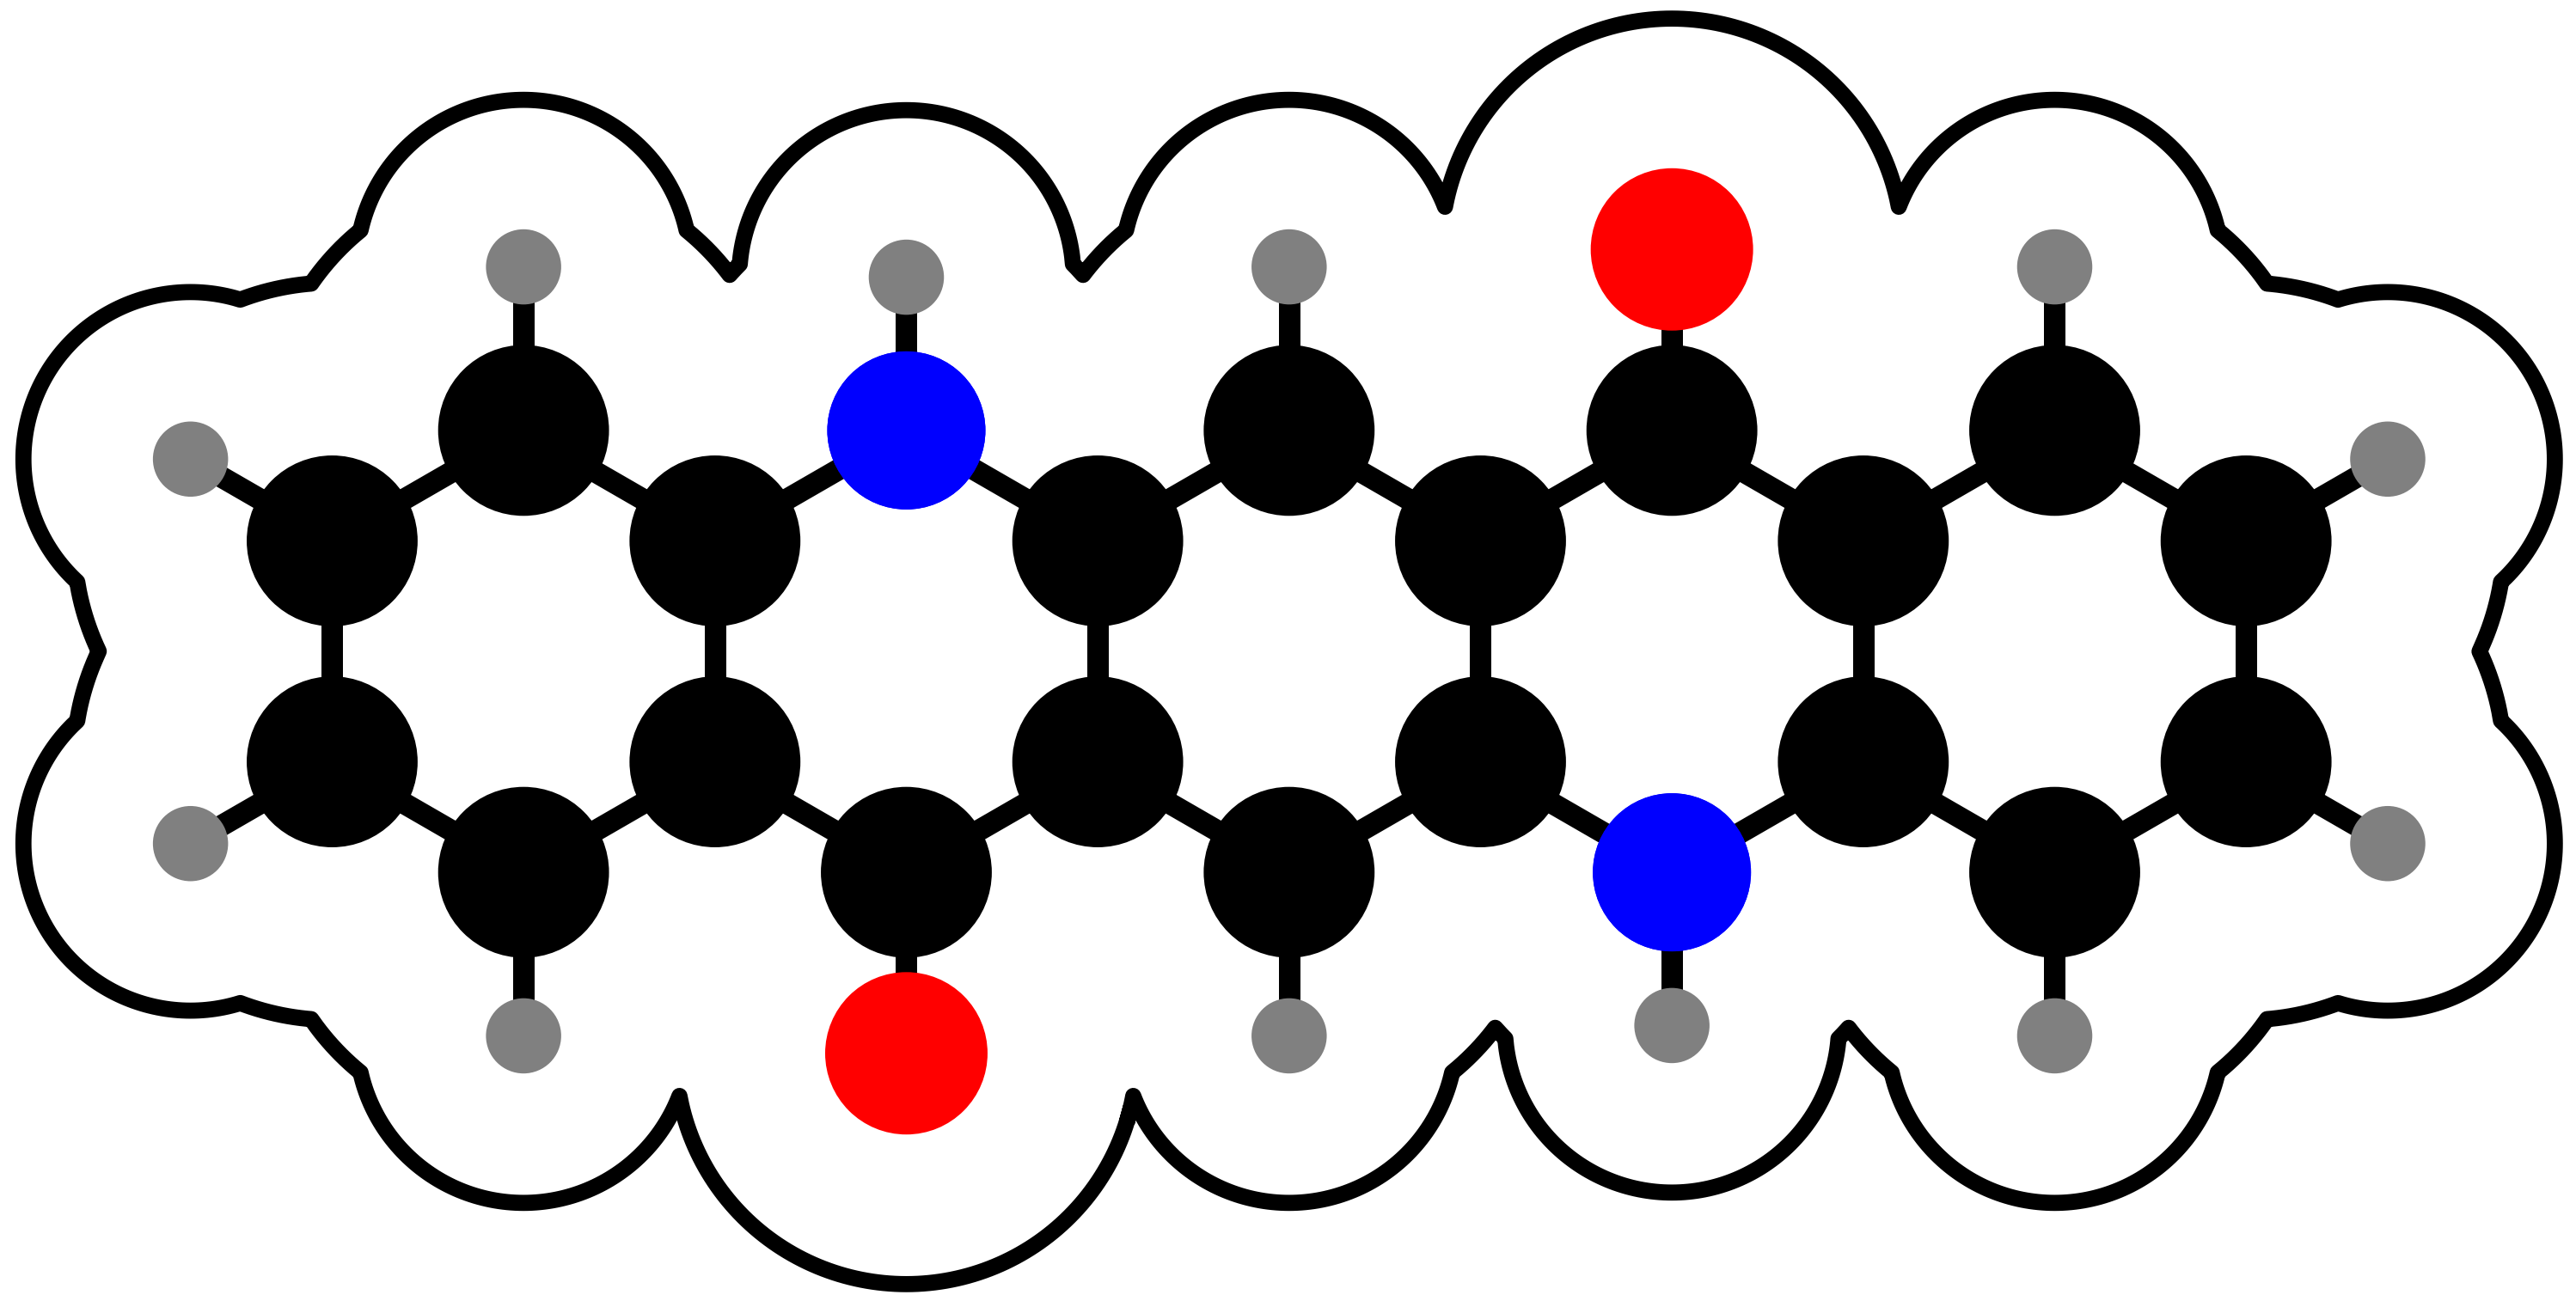
\includegraphics[width=0.8\linewidth]{images/QA_molecule.png}
            \caption{Ball-and-stick model of QA: \\ C: black, H: grey, N: blue, O: red.}
        \end{figure}
    \end{columns}
    
    \vspace{1em}
    \begin{block}{Research Question}
        How do intermolecular hydrogen bonds \& adsorbate-substrate interactions change during phase transitions?
    \end{block}
\end{frame}

\begin{frame}{Known $\alpha$-Phase of QA on Ag(100)}
    \begin{columns}[c]
        \column{0.4\textwidth}
        \textbf{$\alpha$-Phase:}
        \begin{itemize}
            \item Forms at 300~K
            \item \ac{POL} structure
            \item Homochiral 1D chains
            \item Proposed 2 hydrogen bonds per molecule
            \item Metastable phase
        \end{itemize}
        
        \column{0.6\textwidth}
        \begin{figure}
            
\includegraphics[width=0.73\linewidth]{images/literature_alpha.png}
            \caption{$\alpha$-phase of QA on Ag(100).\autocite{Humberg2024}}
        \end{figure}
    \end{columns}
\end{frame}

\begin{frame}{Known $\beta$-Phase of QA on Ag(100)}
    \begin{columns}[c]
        \column{0.4\textwidth}
        \textbf{$\beta$-Phase:}
        \begin{itemize}
            \item Forms after heating to 500~K
            \item Commensurate structure
            \item 2D network with dimers
            \item Proposed 1.5 hydrogen bonds per molecule
            \item Thermodynamically stable
        \end{itemize}
        
        \column{0.6\textwidth}
        \begin{figure}
            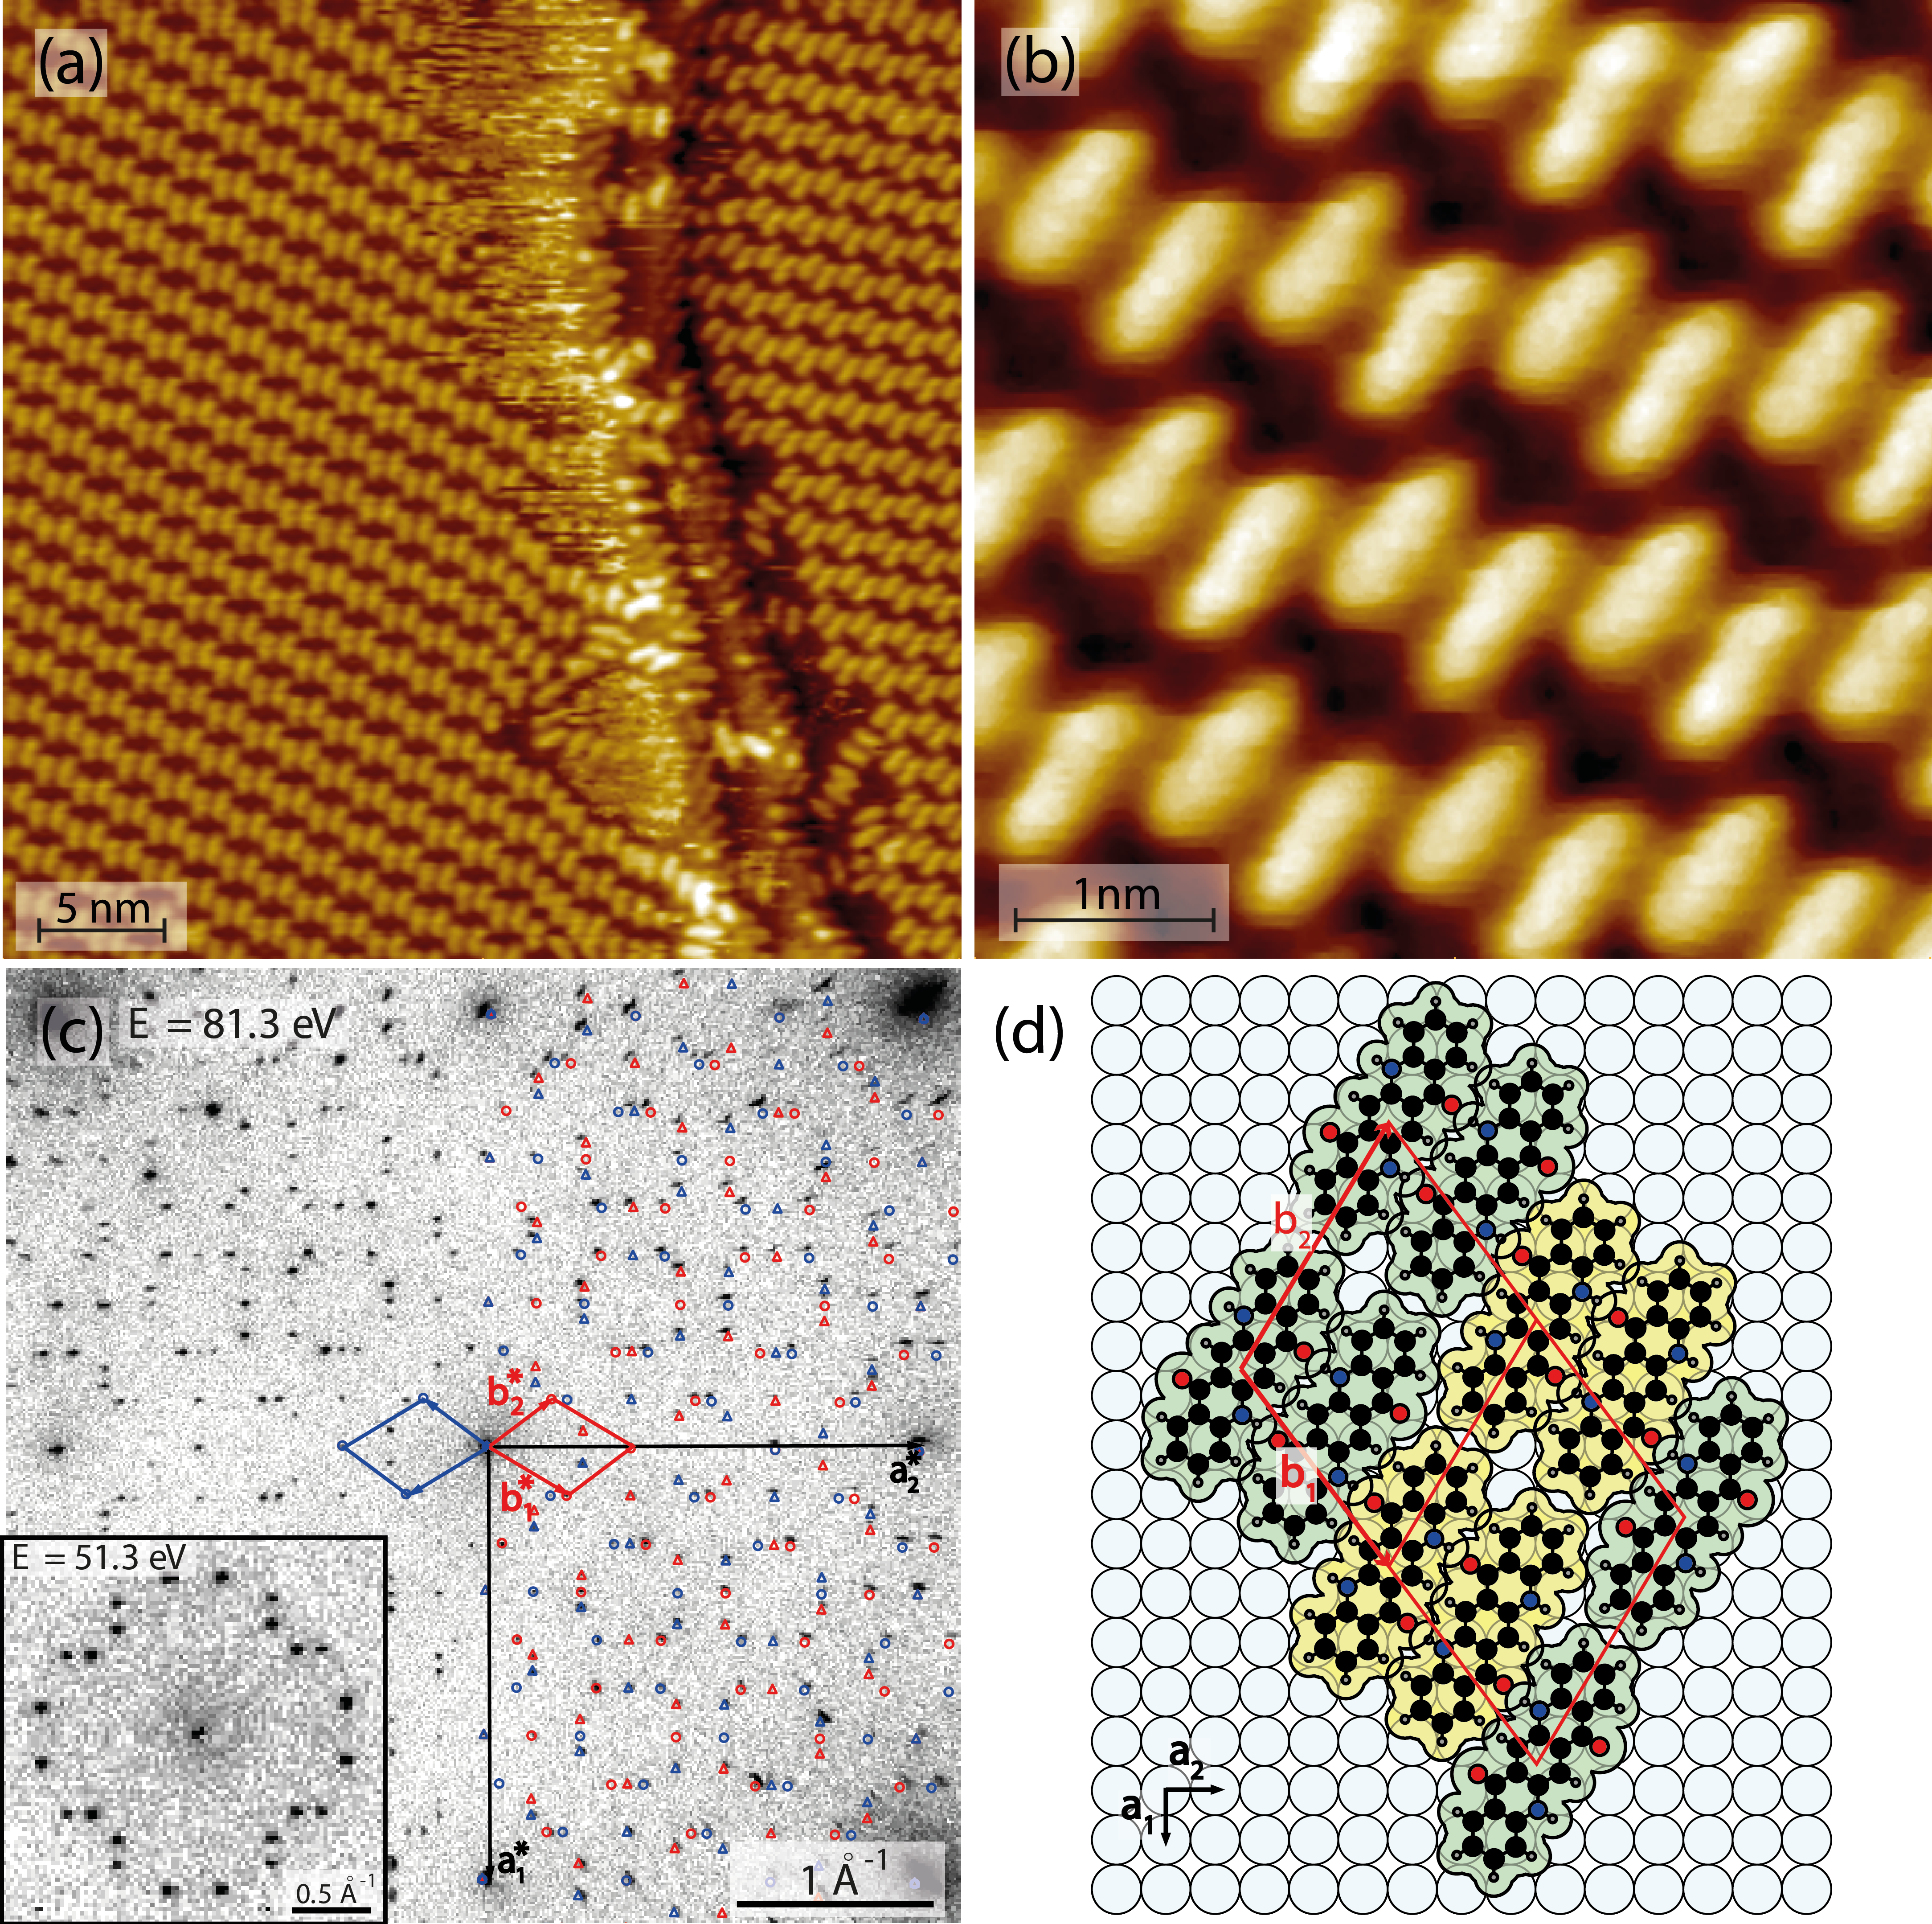
\includegraphics[width=0.73\linewidth]{images/literature_beta.png}
            \caption{$\beta$-phase of QA on Ag(100).\autocite{Humberg2024}}
        \end{figure}
    \end{columns}
\end{frame}

% ================================================================
% THEORY
% ================================================================
\section{Theory}

\begin{frame}{\Acl{XPS}}
    \begin{columns}[c]
        \column{0.6\textwidth}
            \begin{equation*}
                E_{\text{kin}} = h\nu - E_B - \phi_{\text{sample}}
            \end{equation*}

            \vspace{2em}

            \textbf{Key Features:}
            \begin{itemize}
                \item Surface-sensitive ($\sim$ nm depth)
                \item Element-specific core levels
                \item Binding energy reflects local environment
            \end{itemize}

            \column{0.4\textwidth}
            \begin{figure}
                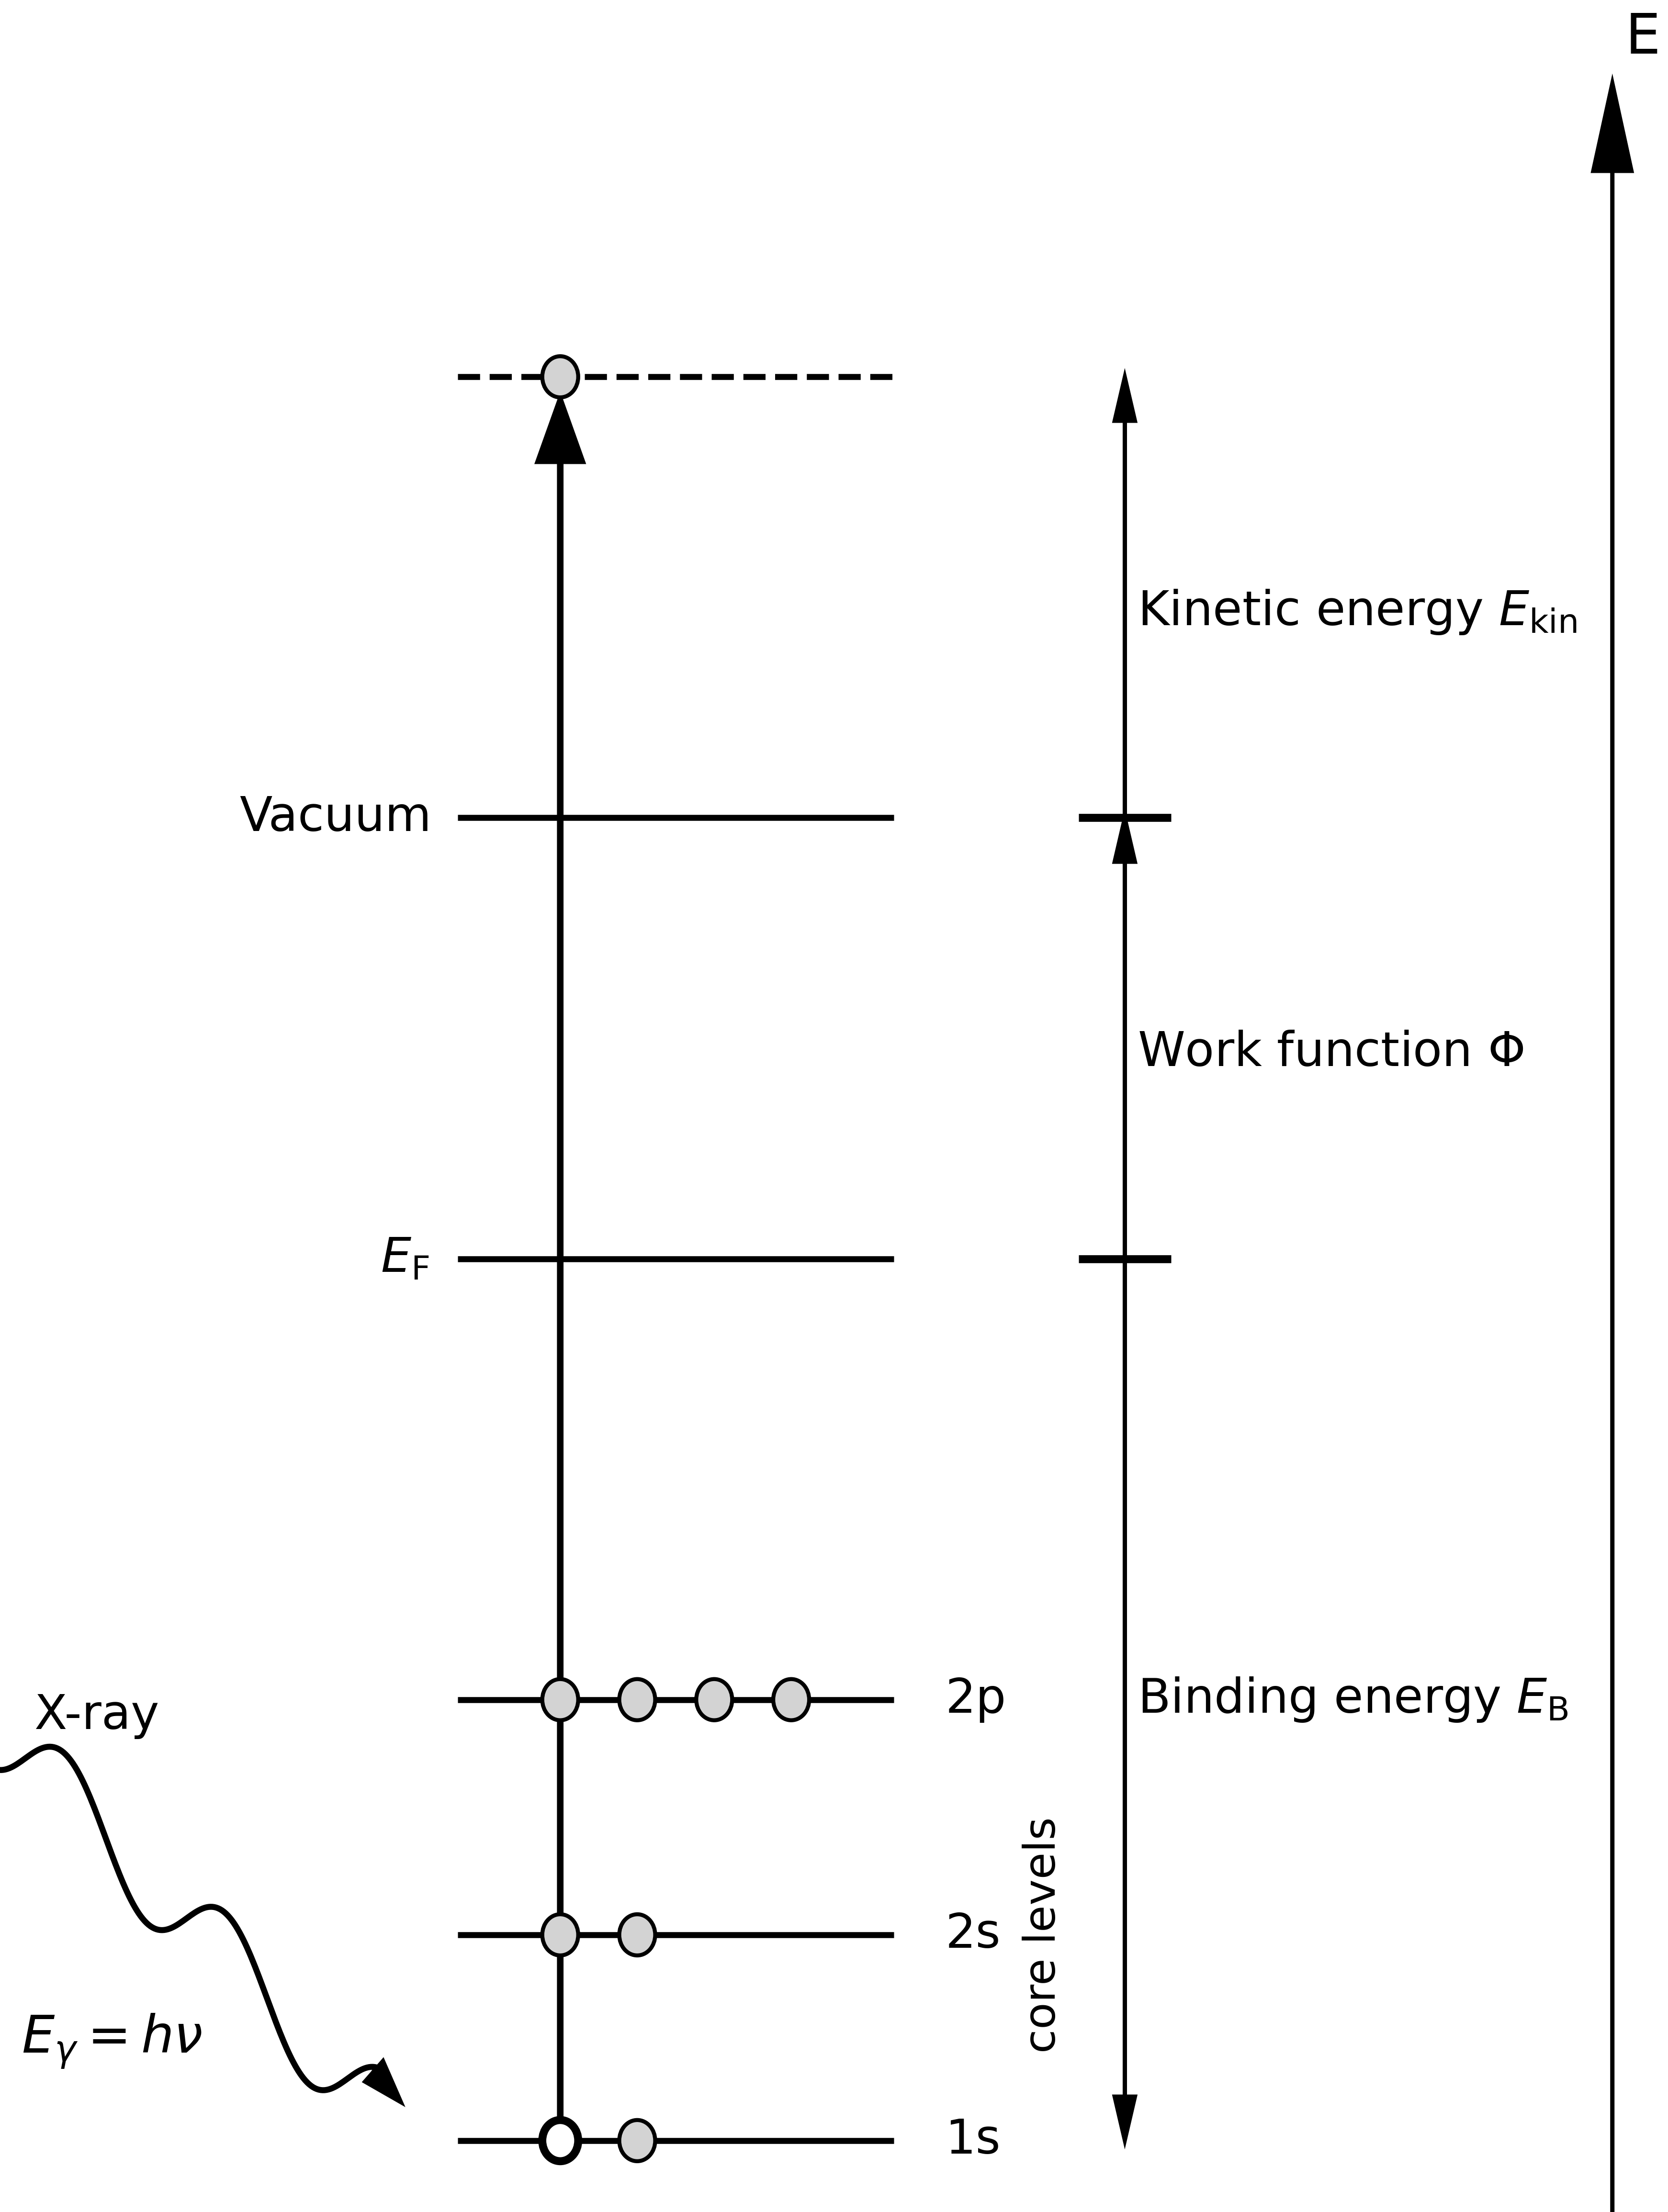
\includegraphics[width=0.87\linewidth]{images/XPS_schematic.png}
            \end{figure}
    \end{columns}
\end{frame}

% ================================================================
% METHODS
% ================================================================
\section{Experimental Methods}

\begin{frame}{Experimental Setup}
        \textbf{Location:} Diamond Light Source (I09 beamline), UK
\begin{columns}[c]
    \column{0.5\textwidth}
    \begin{itemize}
        \item \acs{UHV} chamber ($p\approx 10^{-10}$ mbar)
        \item Synchrotron radiation source
        \item Variable photon energy
    \end{itemize}
    \begin{figure}
        \centering
        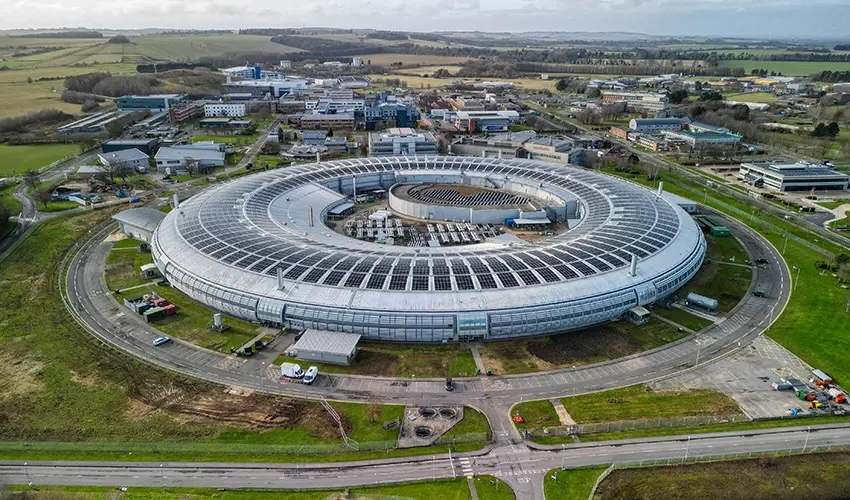
\includegraphics[width=0.9\linewidth]{images/DLS.jpg}
        \caption{Diamond Light Source, UK.\autocite{Diamond2025}}
    \end{figure}

    \column{0.5\textwidth}
    \begin{figure}
        \centering
        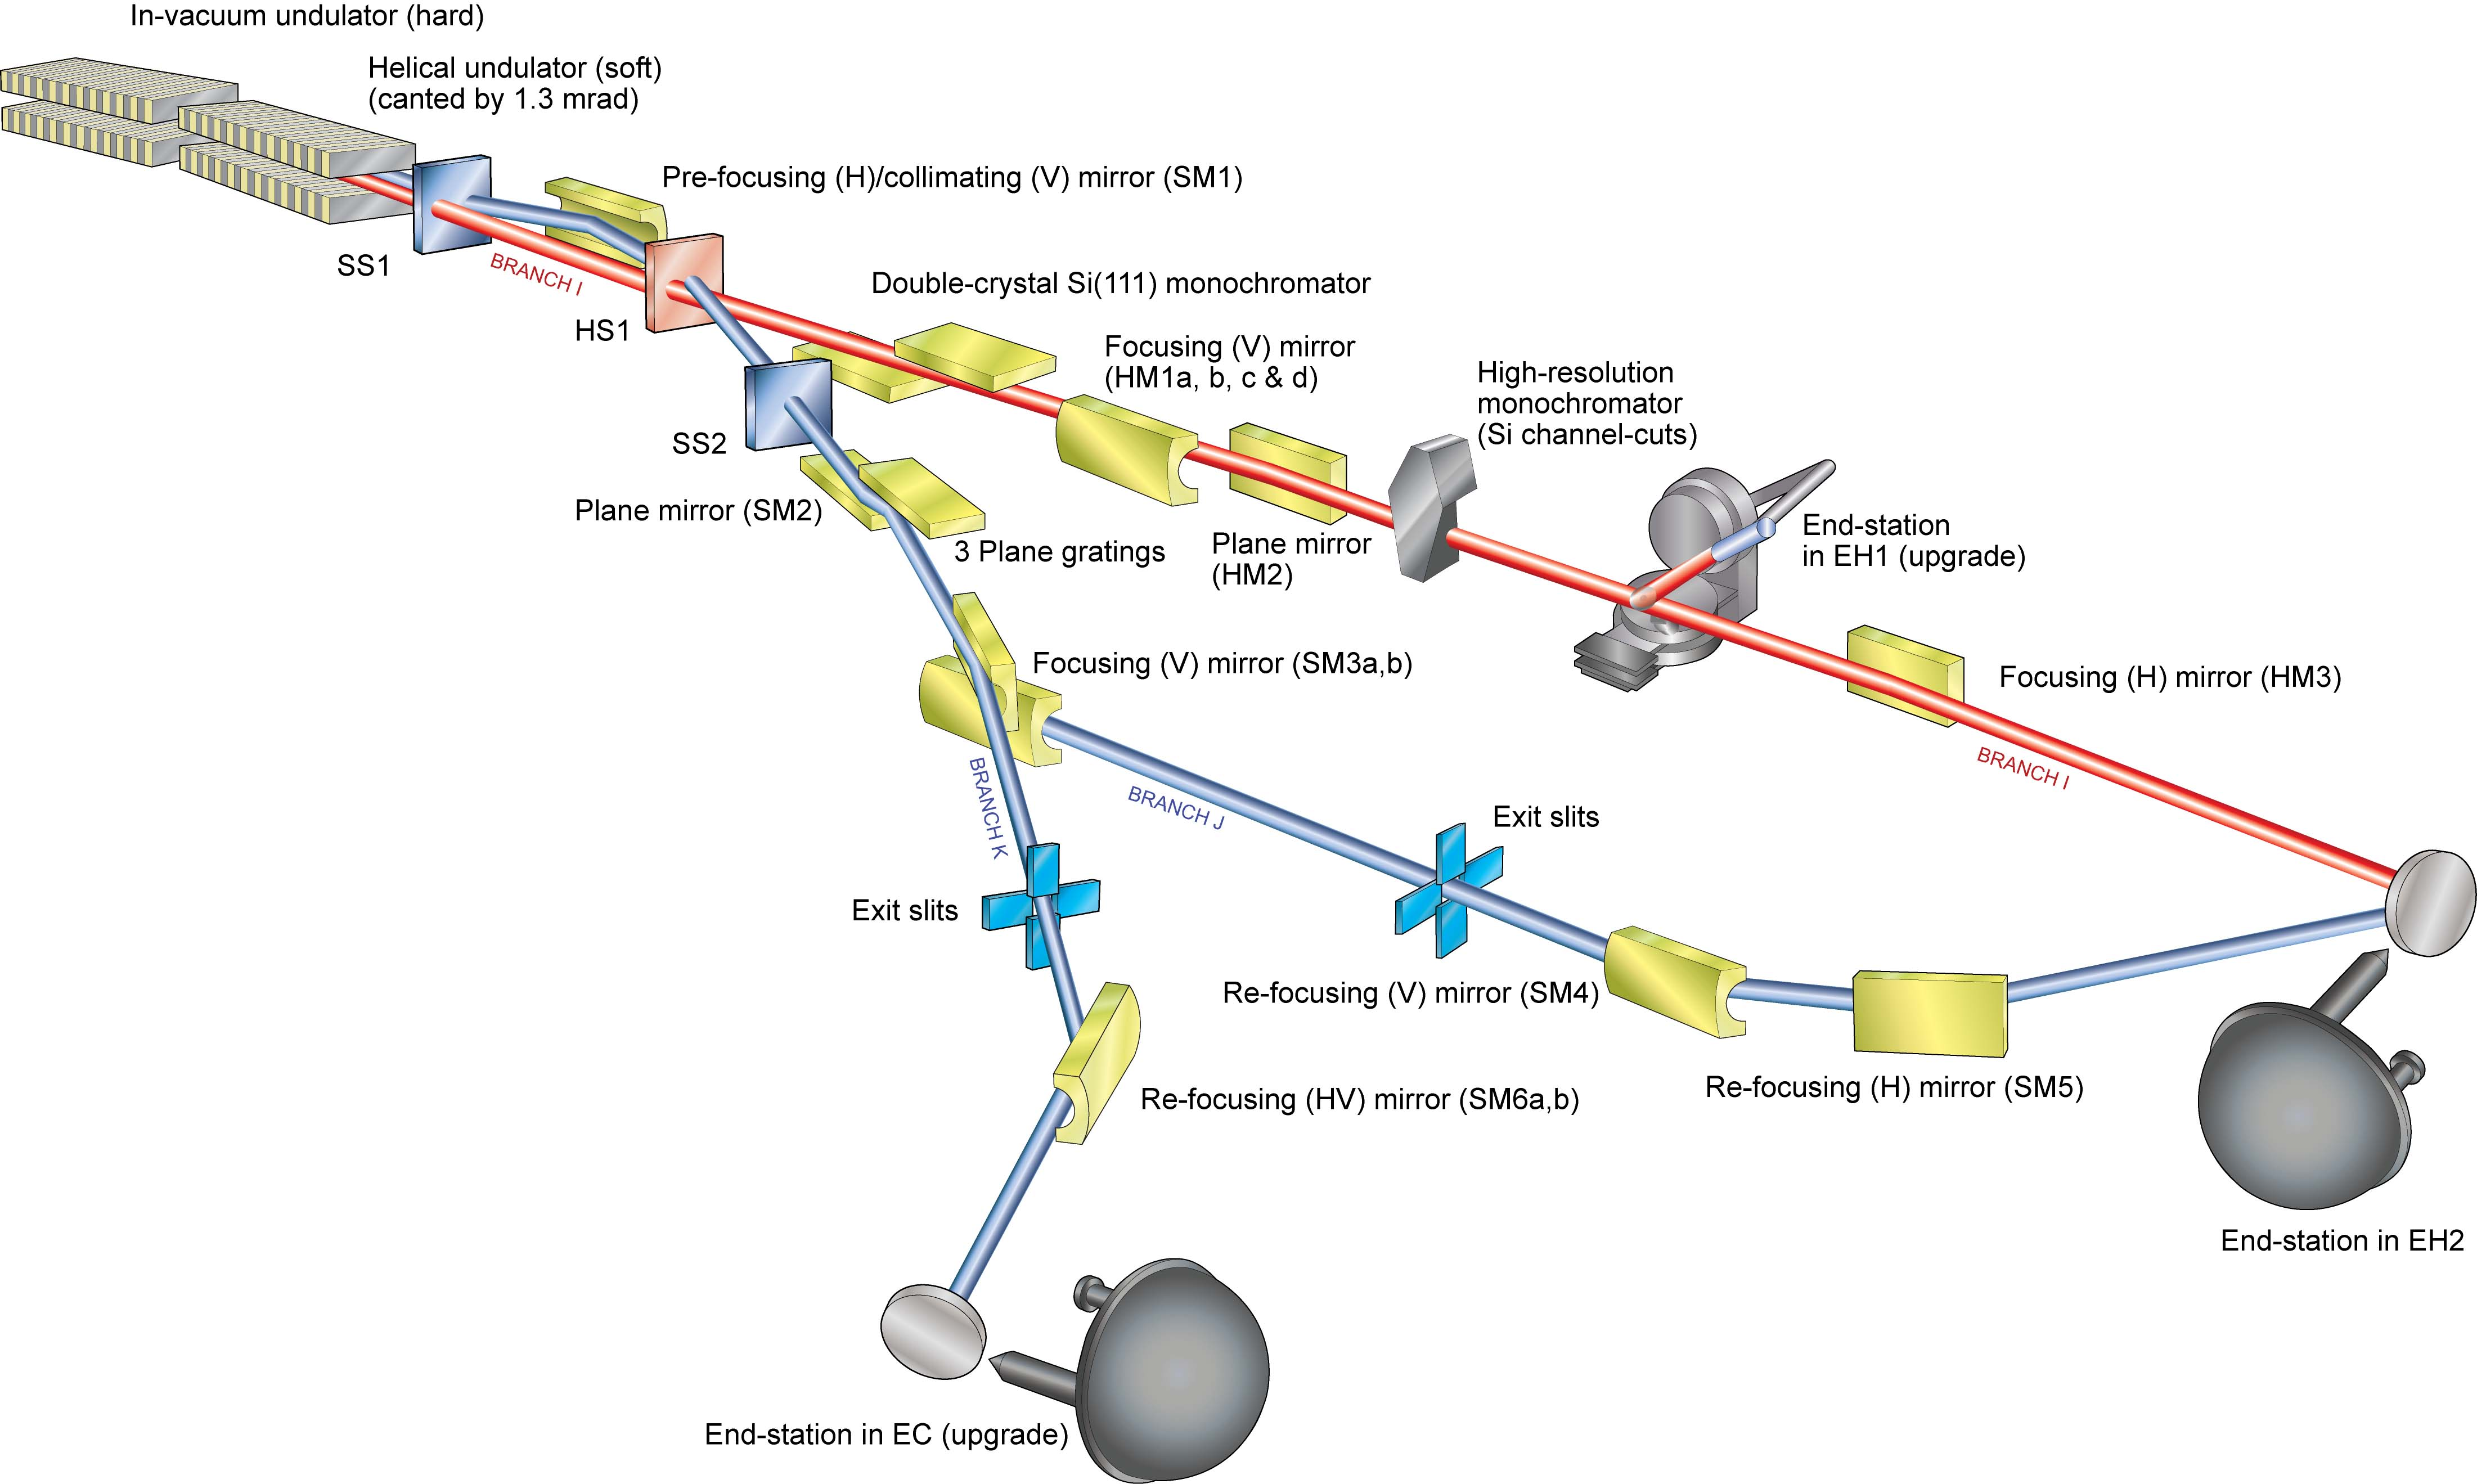
\includegraphics[width=0.8\linewidth]{images/I09.jpg}
        \caption{I09 endstation schematic.\autocite{Diamond2025}}
    \end{figure}
\end{columns}
\end{frame}


% ================================================================
% RESULTS
% ================================================================
\section{Results}

\begin{frame}{C1s \acs{XPS} Spectra}
    \begin{columns}[c]
        \column{0.5\textwidth}
        \begin{figure}
            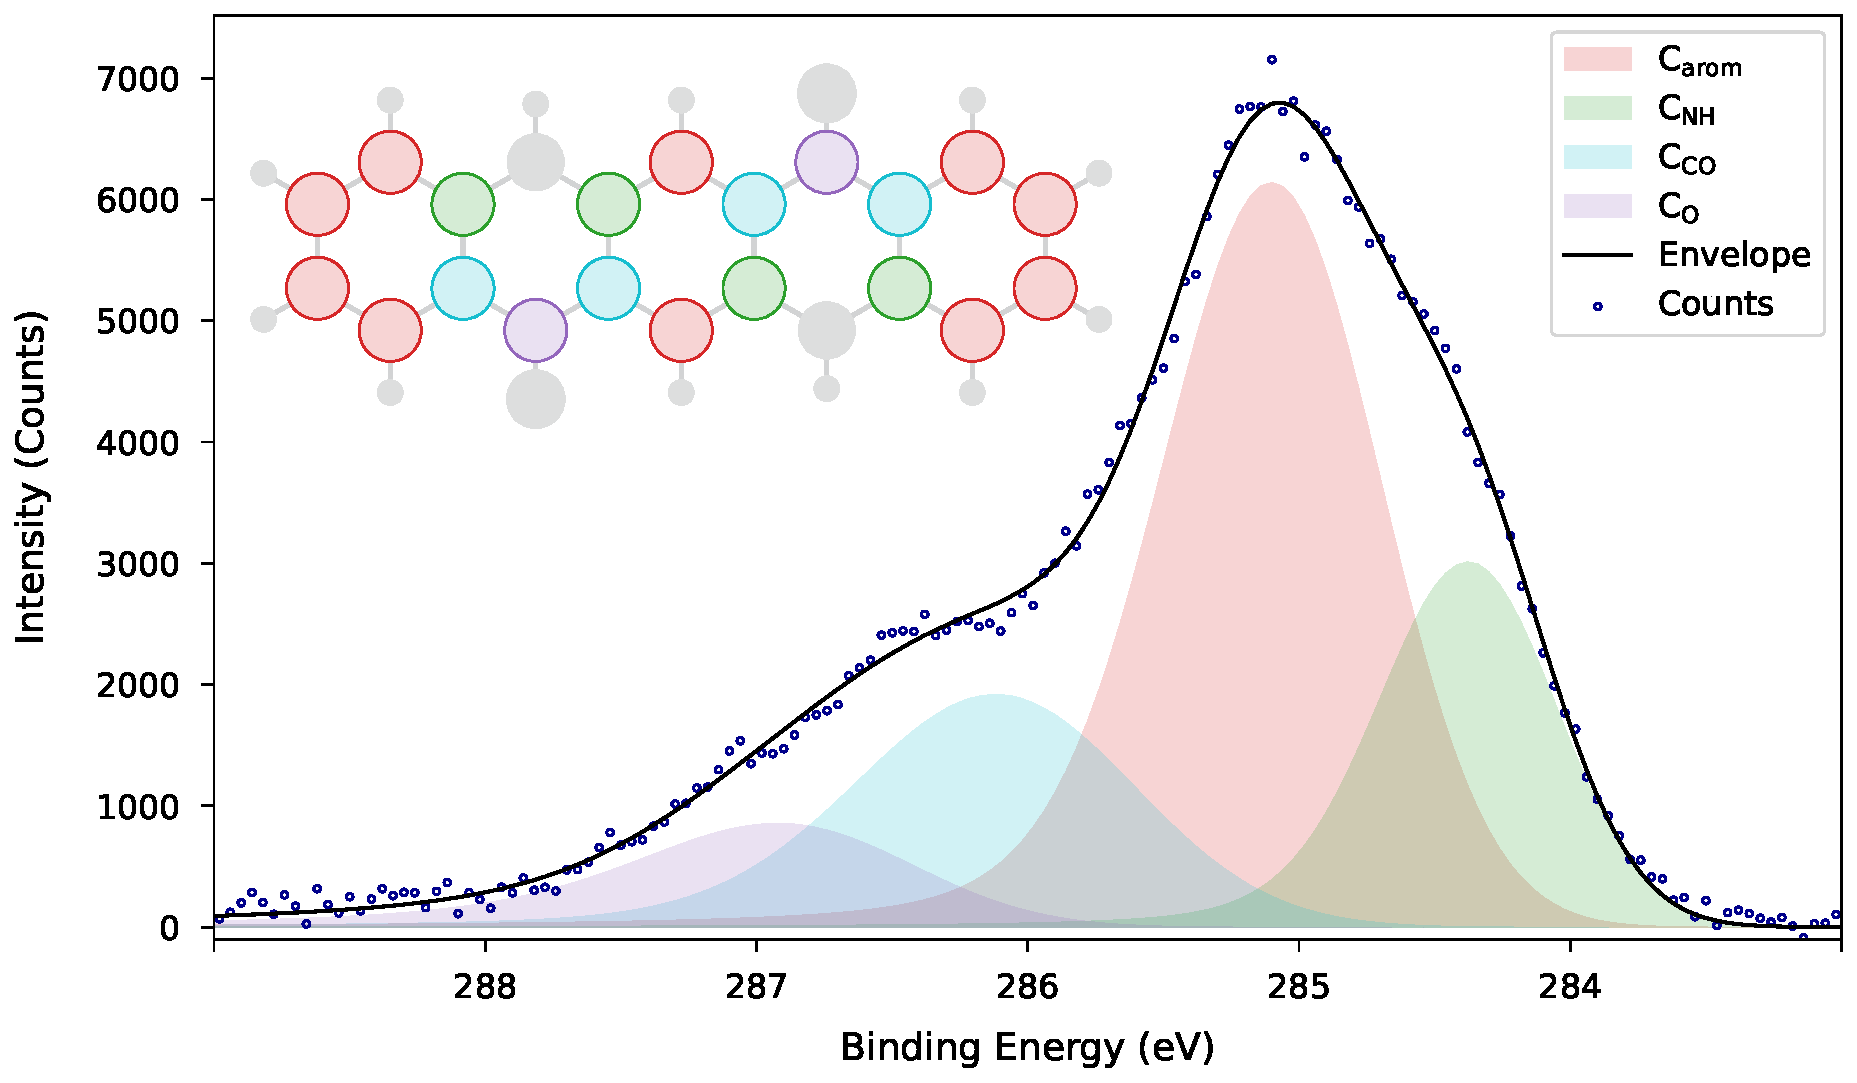
\includegraphics[width=\linewidth]{images/C1s-alpha-P1.pdf}
            \caption{C1s spectrum of $\alpha$-phase.}
        \end{figure}
        
        \column{0.5\textwidth}
        \begin{figure}
            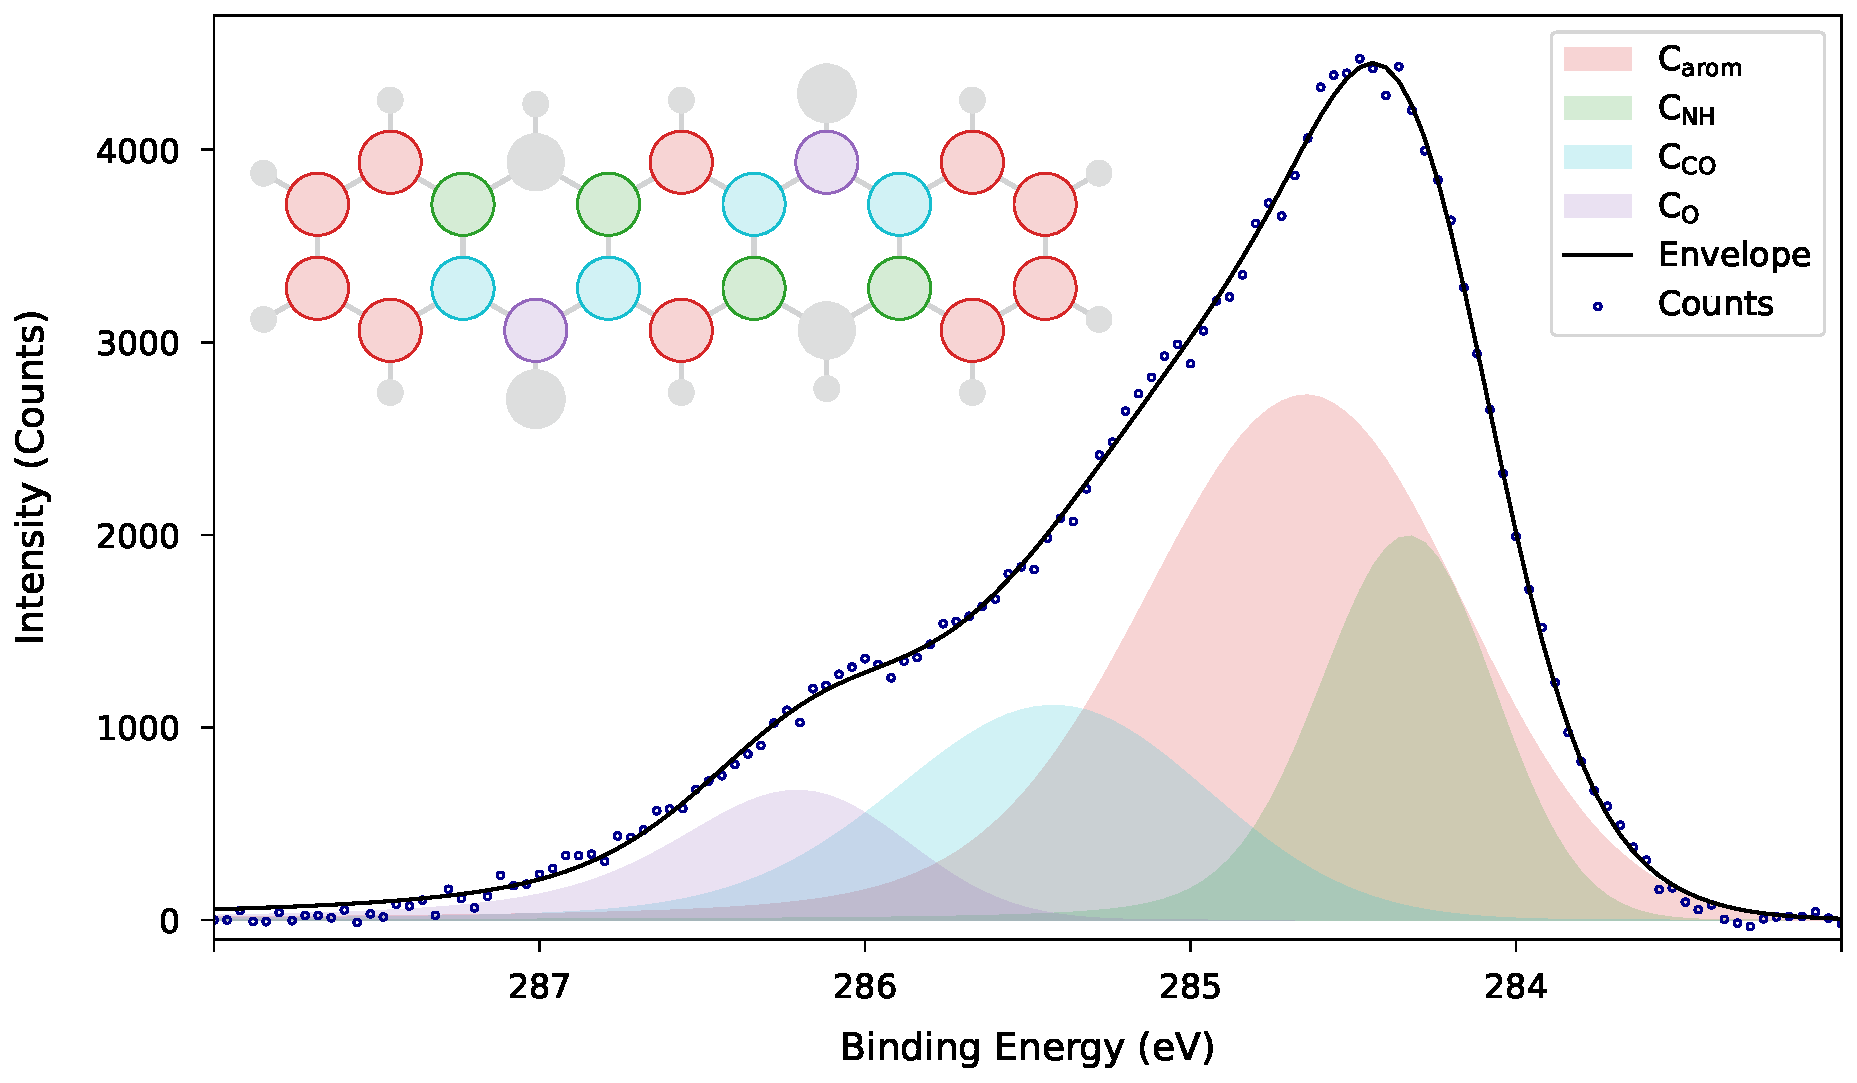
\includegraphics[width=\linewidth]{images/C1s-beta.pdf}
            \caption{C1s spectrum of $\beta$-phase.}
        \end{figure}
    \end{columns}
\end{frame}

\begin{frame}{N1s \acs{XPS} Spectra}
    \begin{columns}[c]
        \column{0.5\textwidth}
        \begin{figure}
            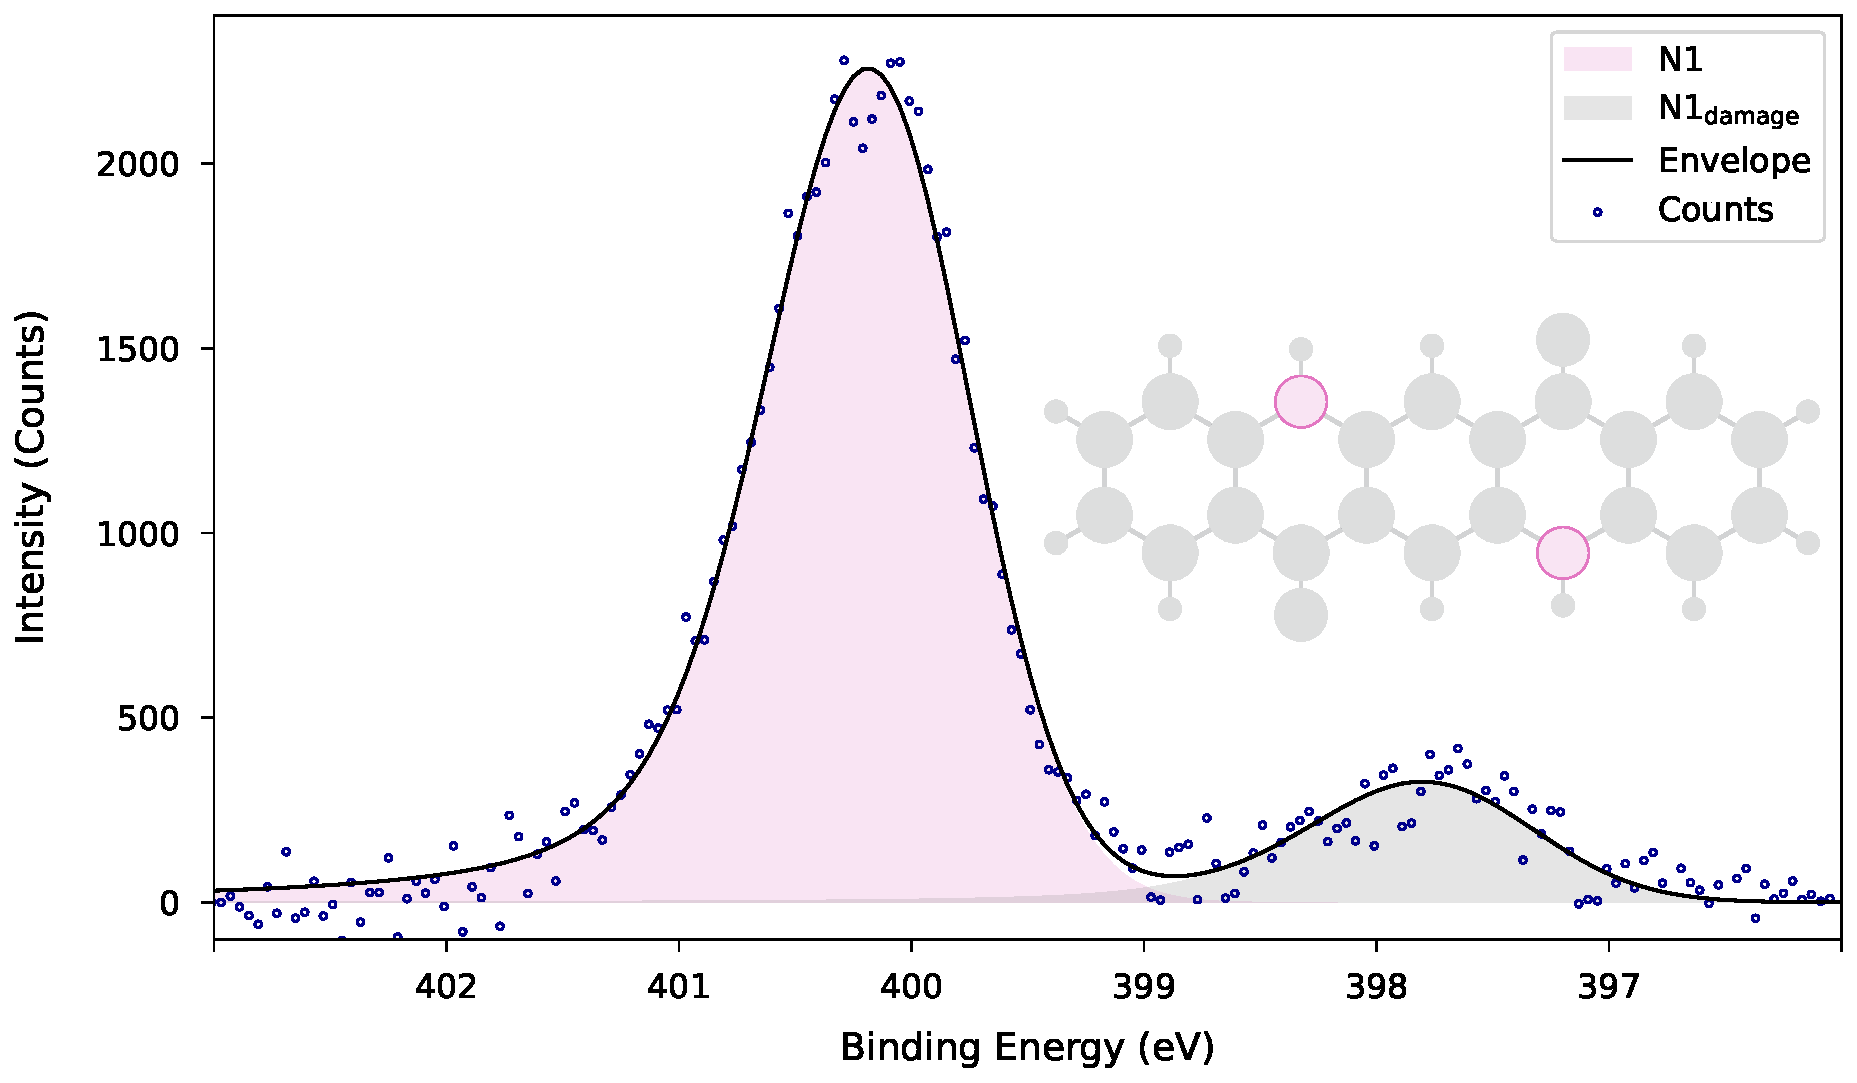
\includegraphics[width=\linewidth]{images/N1s-alpha-P1.pdf}
            \caption{N1s spectrum of $\alpha$-phase.}
        \end{figure}
        
        \column{0.5\textwidth}
        \begin{figure}
            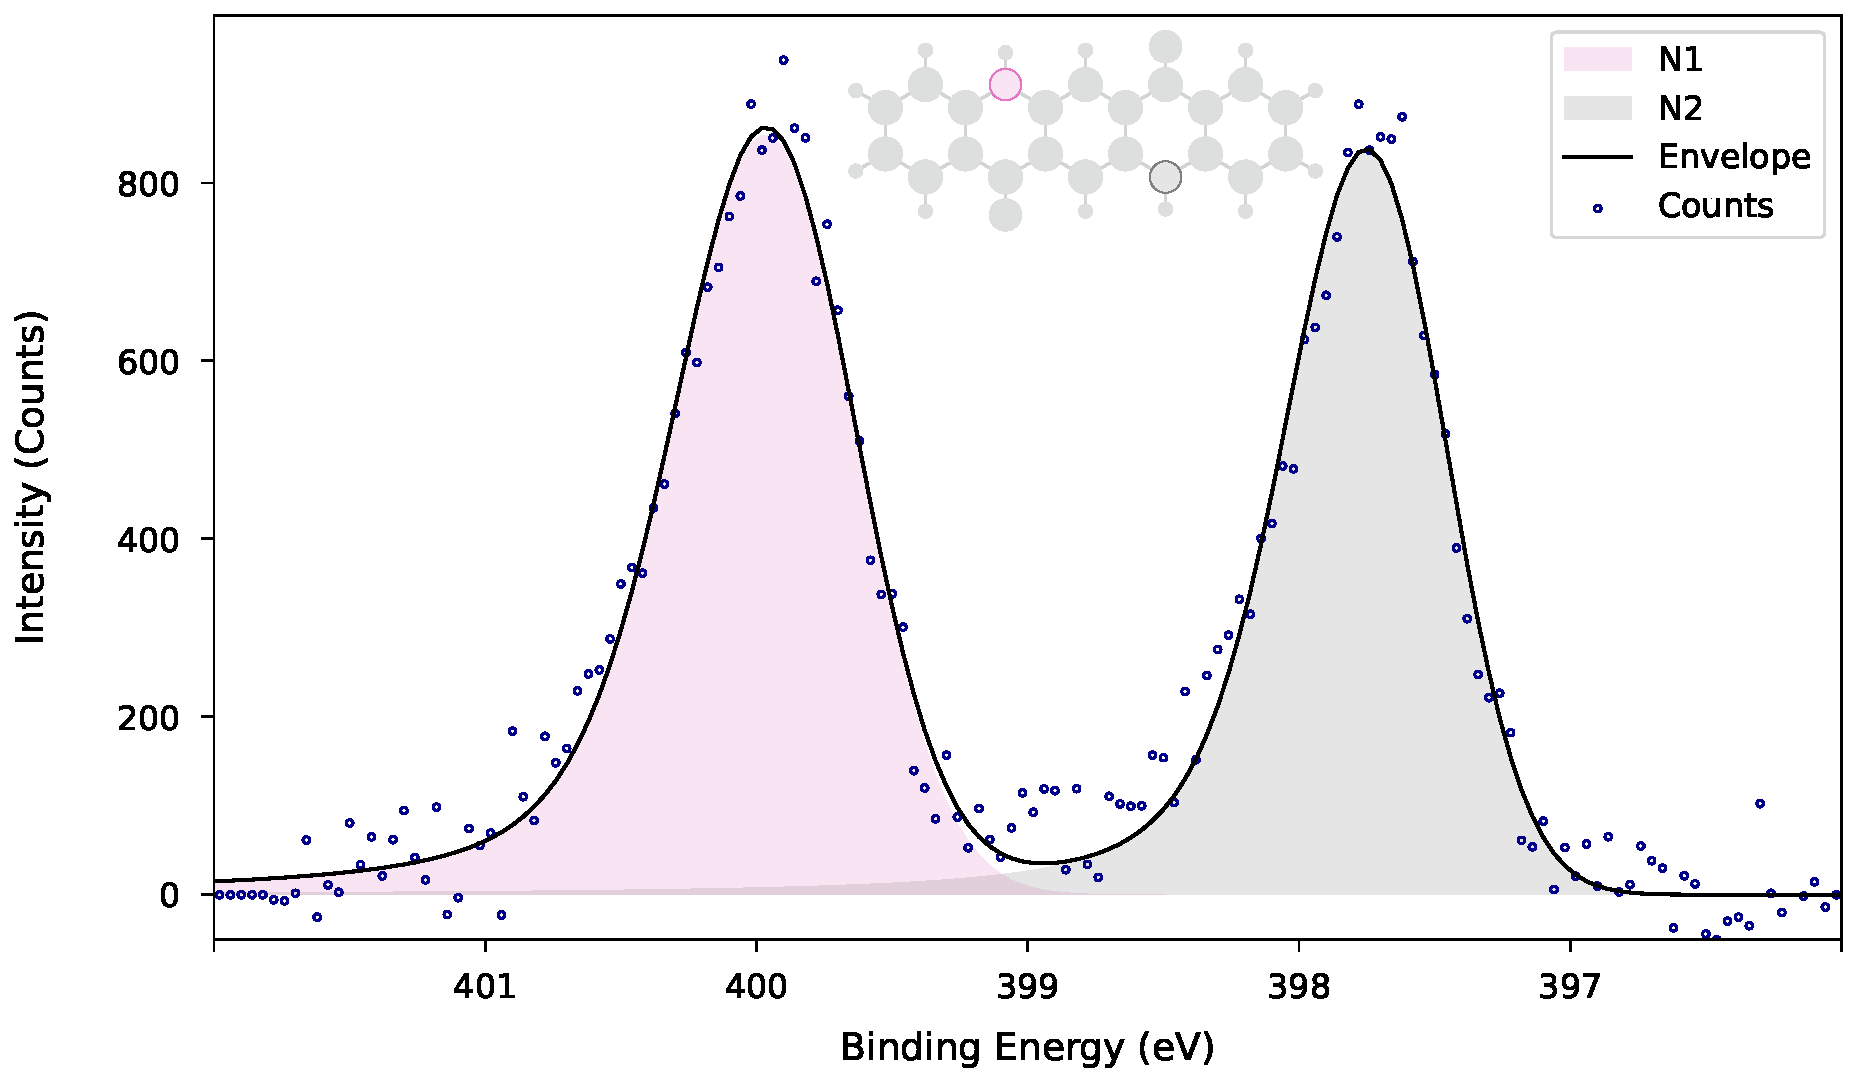
\includegraphics[width=\linewidth]{images/N1s-beta.pdf}
            \caption{N1s spectrum of $\beta$-phase.}
        \end{figure}
    \end{columns}
\end{frame}

\begin{frame}{O1s \acs{XPS} Spectra}
    \begin{columns}[c]
        \column{0.5\textwidth}
        \begin{figure}
            
\includegraphics[width=\linewidth]{images/O1s-alpha-P1.pdf}
            \caption{O1s spectrum of $\alpha$-phase.}
        \end{figure}

        \column{0.5\textwidth}
        \begin{figure}
            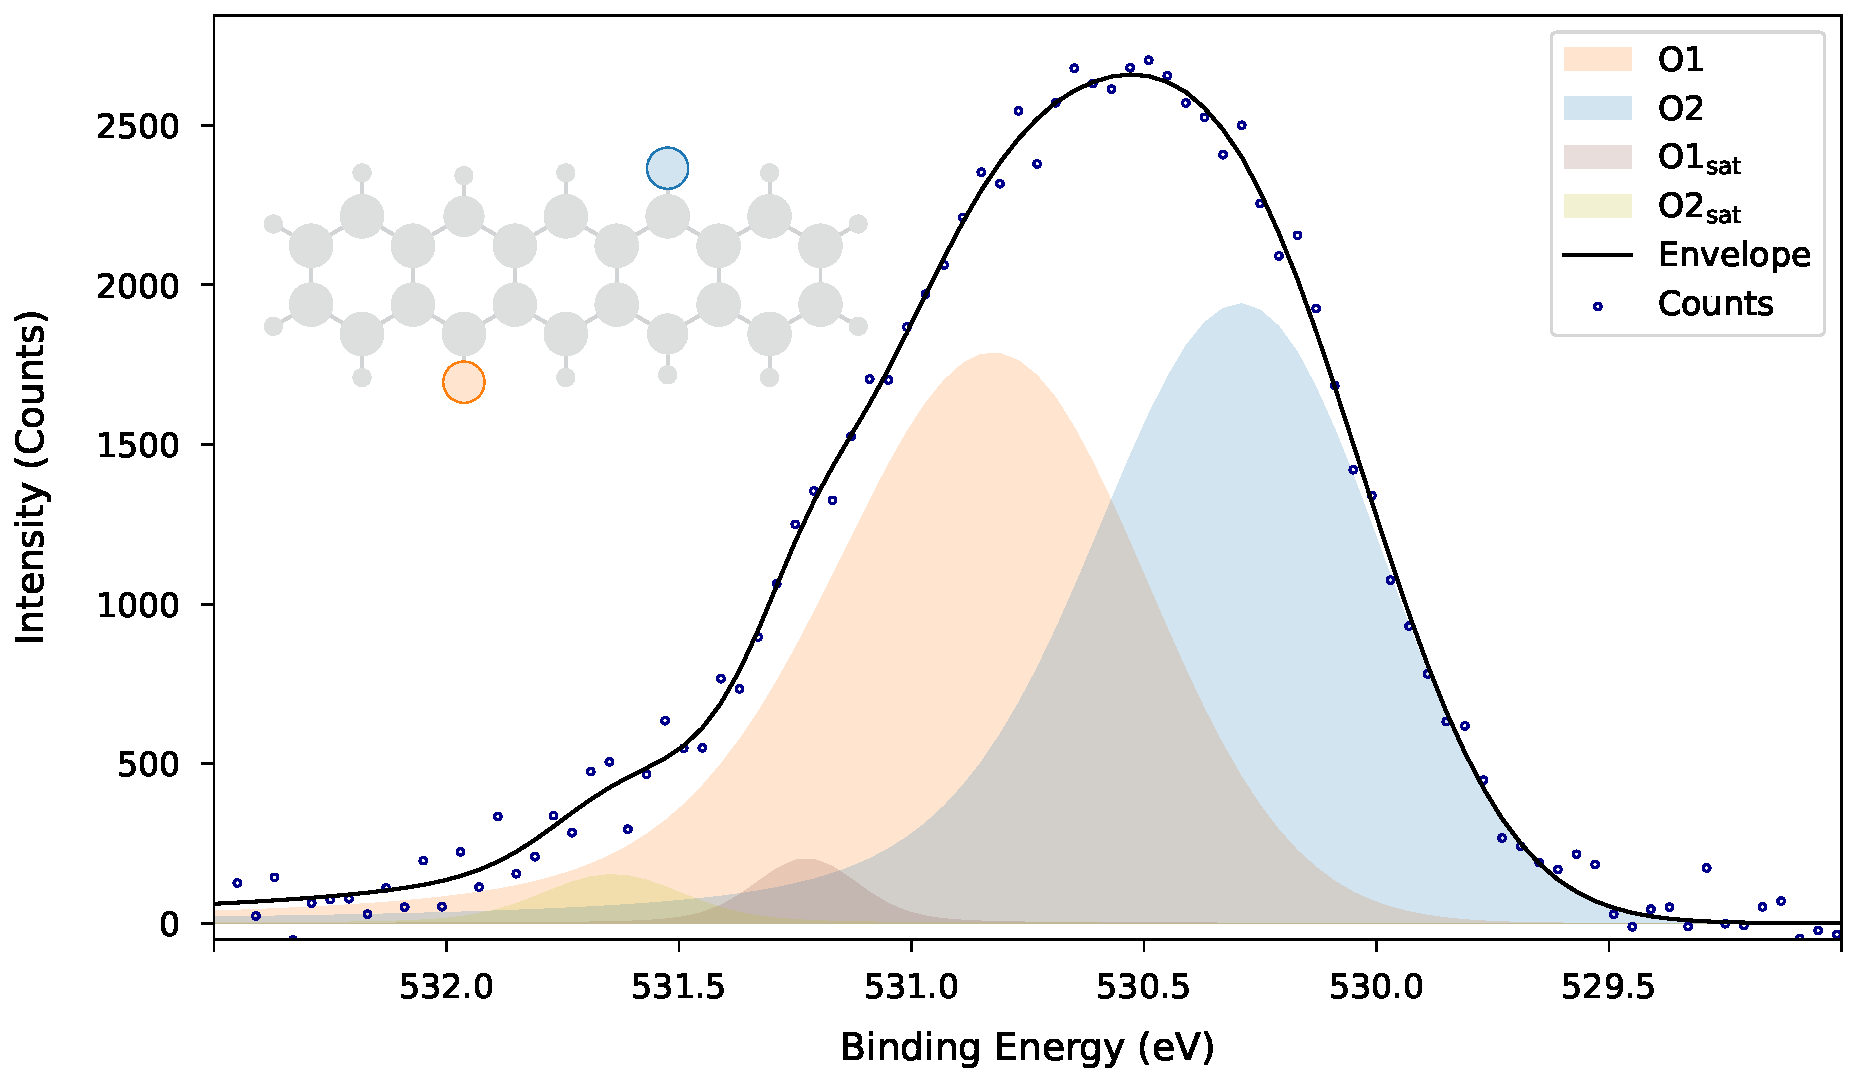
\includegraphics[width=\linewidth]{images/O1s-beta.pdf}
            \caption{O1s spectrum of $\beta$-phase.}
        \end{figure}
        
    \end{columns}
\end{frame}

\begin{frame}{Binding Energy Changes}

    \begin{columns}[c]
        \column{0.5\textwidth}
            \begin{figure}
                \centering
                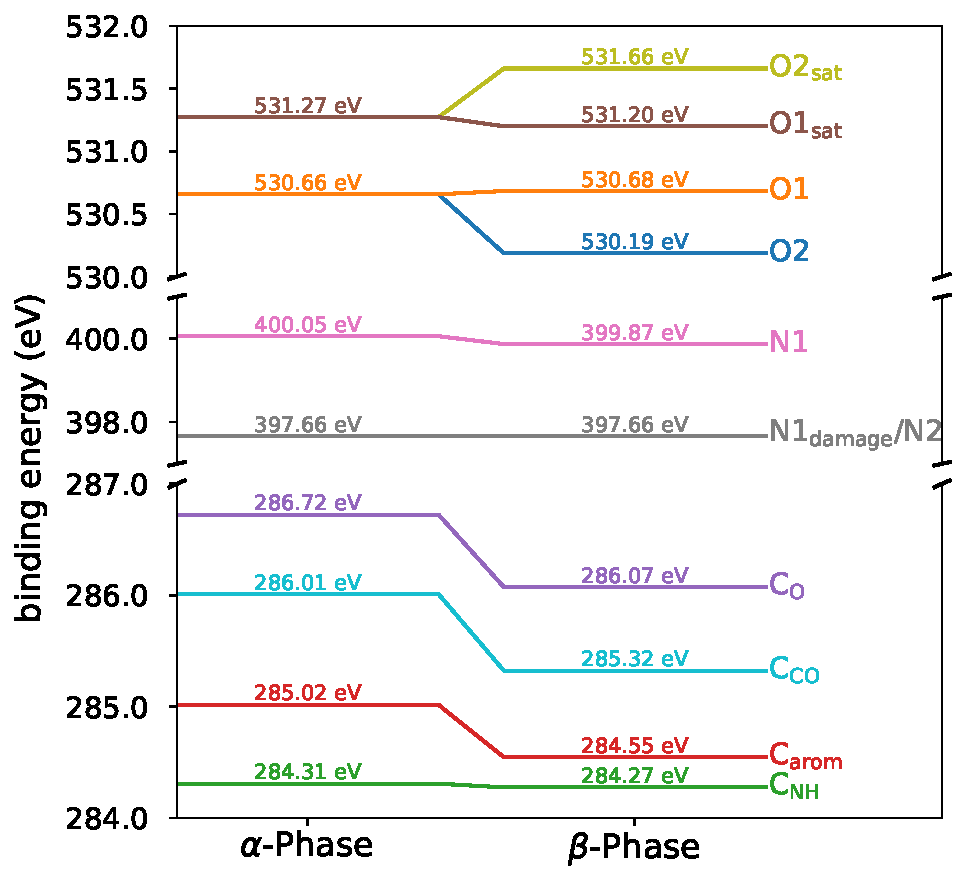
\includegraphics[height=0.78\textheight]{images/phase-shifts.pdf}
                \caption{Binding energy shifts from $\alpha$- to $\beta$-phase.}
            \end{figure}
        \column{0.5\textwidth}
            \begin{itemize}
                \item \textbf{General trend:} Lower BEs in $\beta$-phase \\ $\rightarrow$ stronger surface interaction
                \item \textbf{C1s:} Uniform shifts except for C$_{\text{NH}}$
                \item \textbf{N1s:} Large 2.2 eV shift for N2 component
                \item \textbf{O1s:} 0.5 eV difference between O1 and O2
            \end{itemize}
    \end{columns}
\end{frame}

% ================================================================
% DISCUSSION
% ================================================================
\section{Discussion}

\begin{frame}{Deprotonation Evidence}
    \begin{columns}[c]
        \column{0.5\textwidth}
        \textbf{N1s Shift:}
        \begin{itemize}
            \item 2.2 eV shift matches literature for deprotonated amine group\autocite{Ruano2021,Kang1990,M.Mahat2015}
            \item Similar to beam damage in $\alpha$-phase
        \end{itemize}

        \vspace{0.5cm}

        \textbf{Supporting Evidence:}
        \begin{itemize}
            \item O1s shows 2 distinct environments
            \item One O maintains H-bonding (O1)
            \item Other O loses H-bonding partner (O2)
        \end{itemize}
        
        \column{0.5\textwidth}
        \begin{figure}
            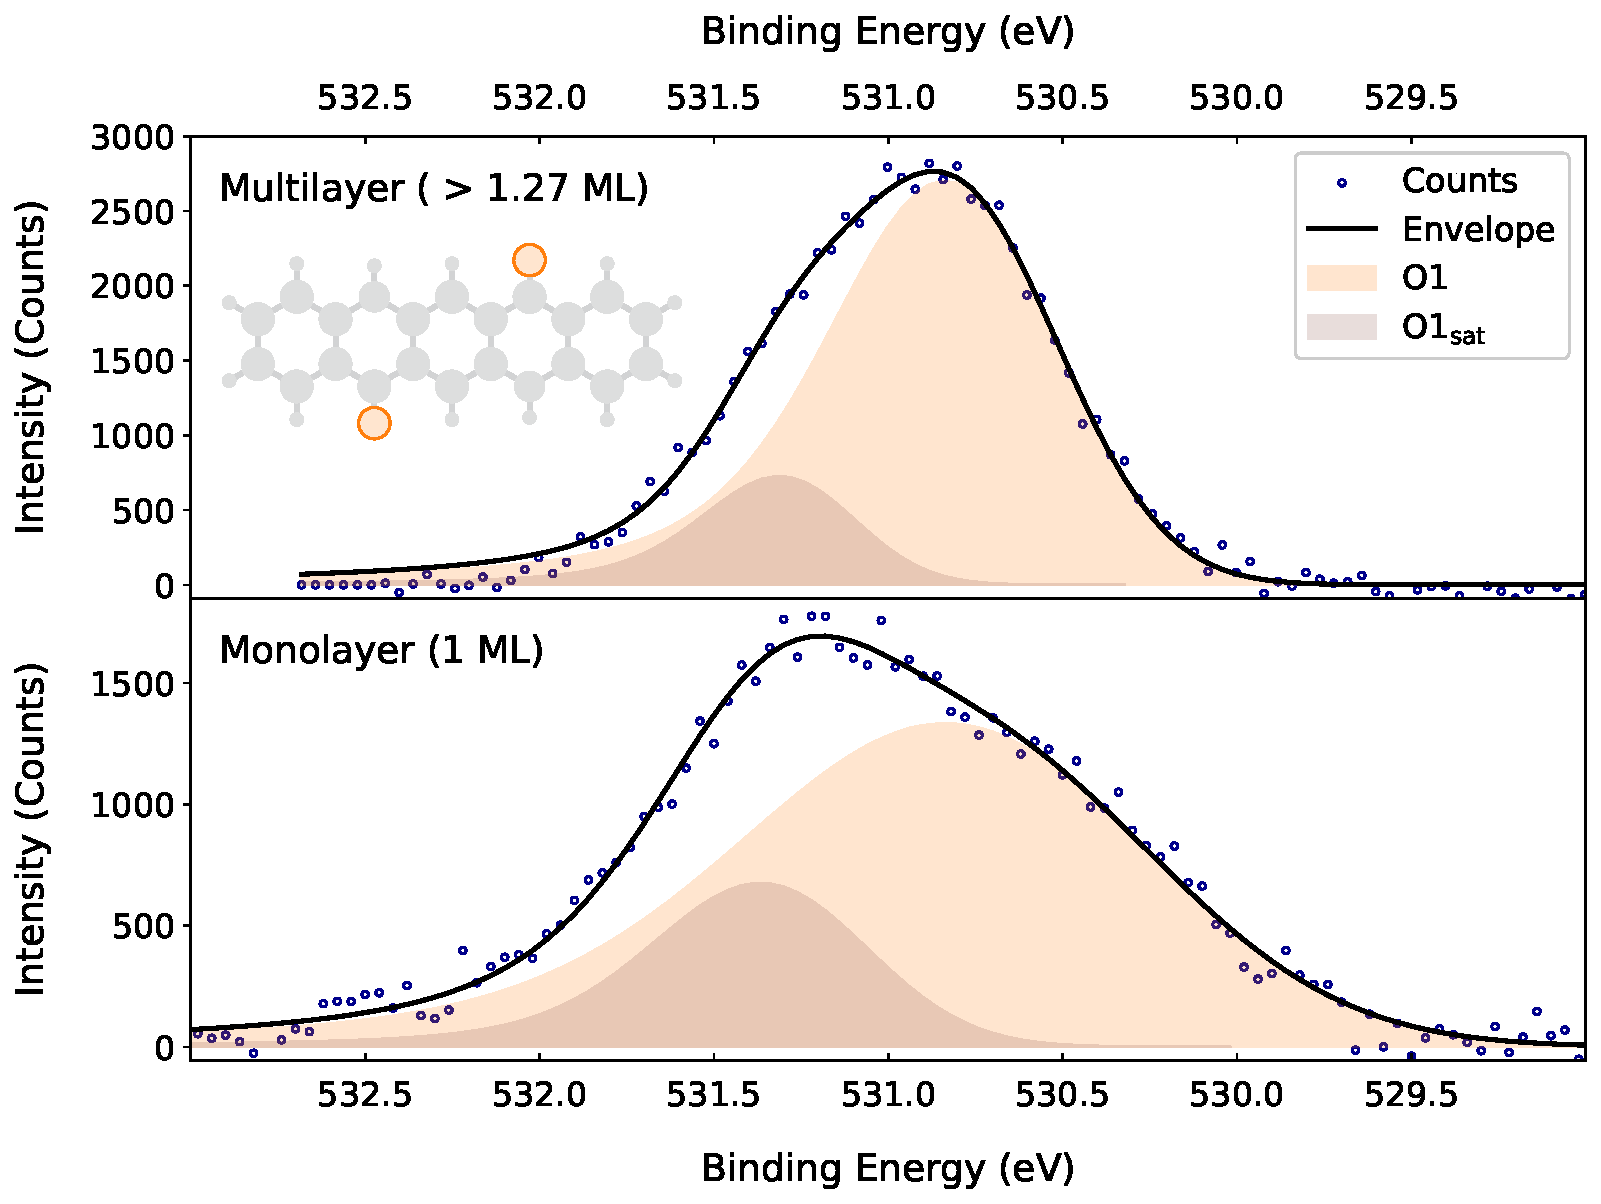
\includegraphics[width=\linewidth]{images/N1s-phase-comparison.pdf}
            \caption{N1s XPS spectra for $\alpha$- \& $\beta$-phase.}
        \end{figure}
    \end{columns}
\end{frame}

\begin{frame}{Key Findings}
    \begin{block}{$\alpha$-Phase}
        \begin{itemize}
            \item Single peaks for N and O atoms $\rightarrow$ equivalent environments
            \item Confirms 2 hydrogen bonds per molecule
        \end{itemize}
    \end{block}
    
    \begin{block}{$\beta$-Phase}
        \begin{itemize}
            \item 2 distinct N \& 2 distinct O environments (1:1 area ratio)
            \item Large N1s shift suggests deprotonation of 1 amine group
            \item Evidence for only 1 hydrogen bond per molecule
        \end{itemize}
    \end{block}
    
    \begin{alertblock}{New Interpretation}
        Phase transition involves deprotonation of 1 amine group per molecule!
    \end{alertblock}
\end{frame}

\begin{frame}{Structure Models: $\alpha$- vs. $\beta$-Phase}
    \begin{columns}[c]
        \column{0.49\textwidth}
        \begin{figure}
            \centering
            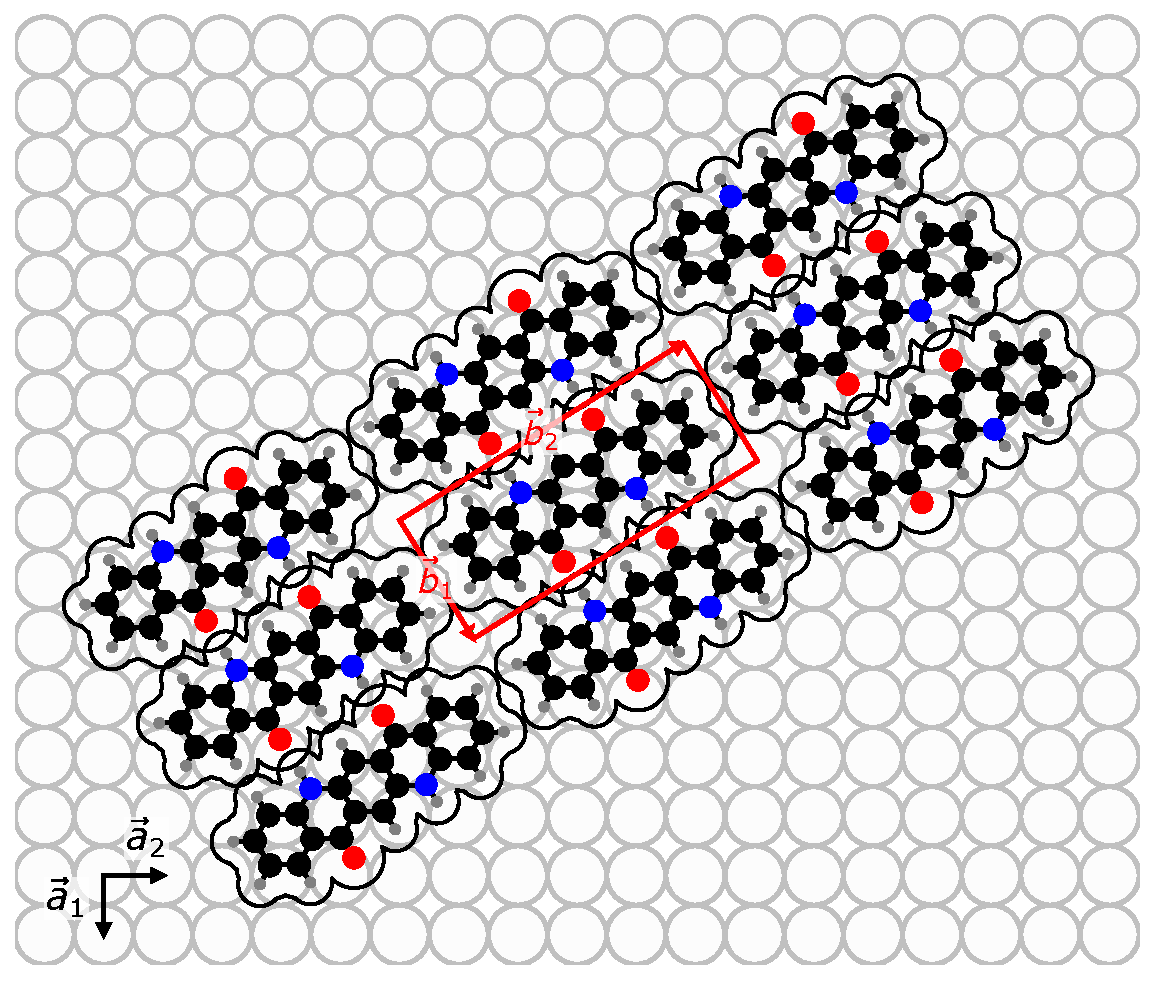
\includegraphics[height=0.7\textheight]{images/QA-alpha-Ag(100).pdf}
            \caption{$\alpha$-phase: 2 H-bonds per molecule, all N and O atoms equivalent}
        \end{figure}
        
        \column{0.49\textwidth}
        \begin{figure}
            \centering
            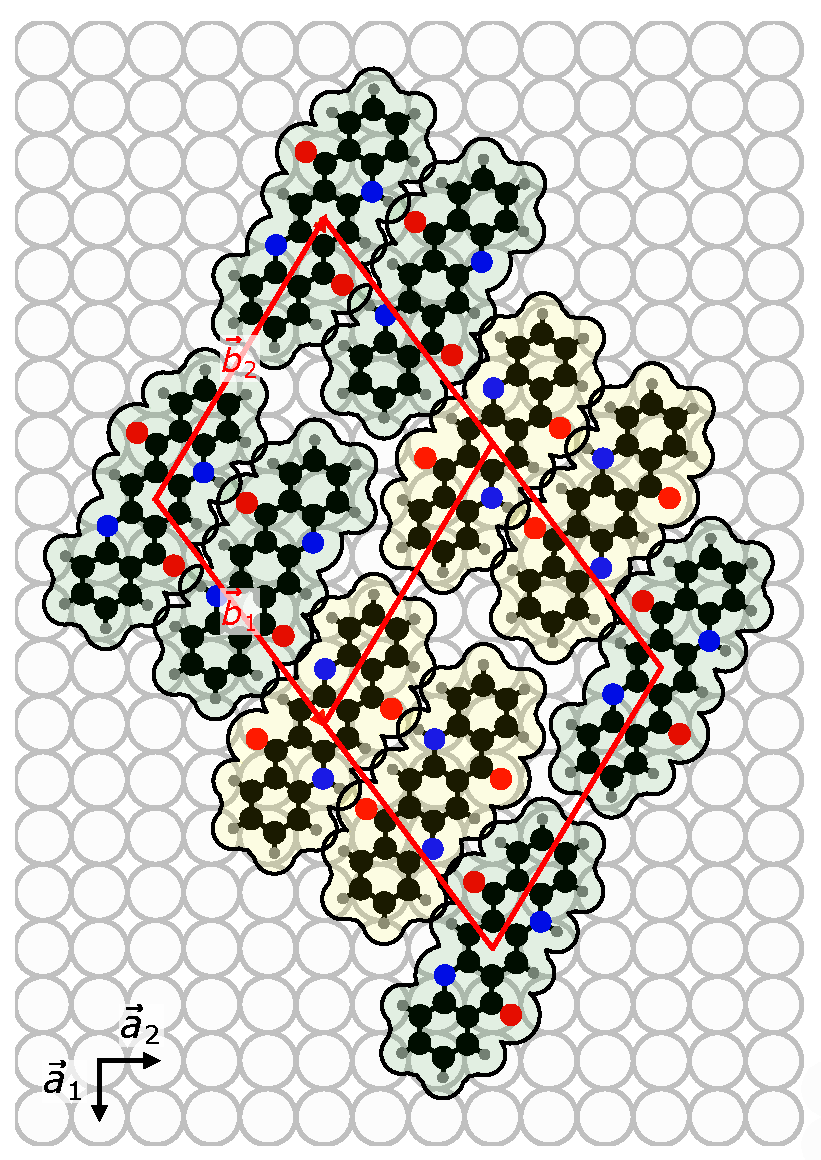
\includegraphics[height=0.7\textheight]{images/QA-beta-Ag(100)-Version1.pdf}
            \caption{$\beta$-phase: 1 H-bond per molecule, one N deprotonated}
        \end{figure}
    \end{columns}
\end{frame}

% ================================================================
% CONCLUSION
% ================================================================
\section{Conclusion \& Outlook}

\begin{frame}{Summary of Main Results}
    \begin{enumerate}
        \item \textbf{Confirmed $\alpha$-phase structure:}
        \begin{itemize}
            \item 2 hydrogen bonds per molecule
            \item All N \& all O atoms have equivalent environments
            \item Consistent with existing structure model
        \end{itemize}
        
        \item \textbf{Revised $\beta$-phase understanding:}
        \begin{itemize}
            \item 1 hydrogen bond per molecule (not 1.5)
            \item 1 deprotonated amine group per molecule, 2 distinct N \& 2 distinct O environments
            \item Requires new structure model
        \end{itemize}
        
        \item \textbf{Phase transition:}
        \begin{itemize}
            \item Deprotonation of amine group
            \item Stronger molecule-surface interactions in $\beta$-phase
        \end{itemize}
    \end{enumerate}
    
    \begin{alertblock}{Key Impact}
        New insights into molecular interactions and phase behavior of \acs{QA} on the Ag(100) surface, including evidence for deprotonation during phase transition.
    \end{alertblock}
\end{frame}

\begin{frame}{Future Perspectives}
    \begin{block}{Follow-up Studies}
        \begin{itemize}
            \item \textbf{\Ac{NIXSW}:} Determine exact adsorption heights and sites
            \item \textbf{Mass spectrometry:} Detect H$_2$ evolution during phase transition
            \item \textbf{Other derivatives:} Study similar systems, e.g. FQA
        \end{itemize}
    \end{block}
\end{frame}

% ================================================================
% BACKUP/APPENDIX
% ================================================================
\appendix

\begin{frame}[allowframebreaks]{References}
    \printbibliography
\end{frame}

\begin{frame}{Thank you!}
    \centering
    \vspace{1cm}
    \Huge Thank you for your attention!
    
    \vspace{2em}
    \Large \textbf{Questions?}
    
    \vspace{2em}
    \normalsize
    \textbf{Lucas Hirschfeld}\\
    Clausius Institute, University of Bonn\\
    \texttt{hirschfeld@pc.uni-bonn.de}

    \begin{tikzpicture}[remember picture,overlay]
    \node[anchor=south east, xshift=-0.2cm, yshift=0.2cm] at (current page.south east) {
        
\includegraphics[height=0.8cm]{images/logo.png}
    };
    \end{tikzpicture}
\end{frame}

% ================================================================
% BACKUP SLIDES
% ================================================================

\begin{frame}{Quinacridone Properties}
    \begin{columns}[c]
        \column{0.6\textwidth}
        \textbf{Chemical Properties:}
        \begin{itemize}
            \item Formula: \ch{C20H12N2O2}
            \item Prochiral organic molecule
            \item Highly conjugated $\pi$-system
            \item Symmetry group: $C_{2h}$
        \end{itemize}
        
        \textbf{Applications:}
        \begin{itemize}
            \item Pigment in industry (Violet 19)
            \item Well-defined surface structures
            \item Organic electronics components
        \end{itemize}
        
        \column{0.4\textwidth}
        \begin{figure}
            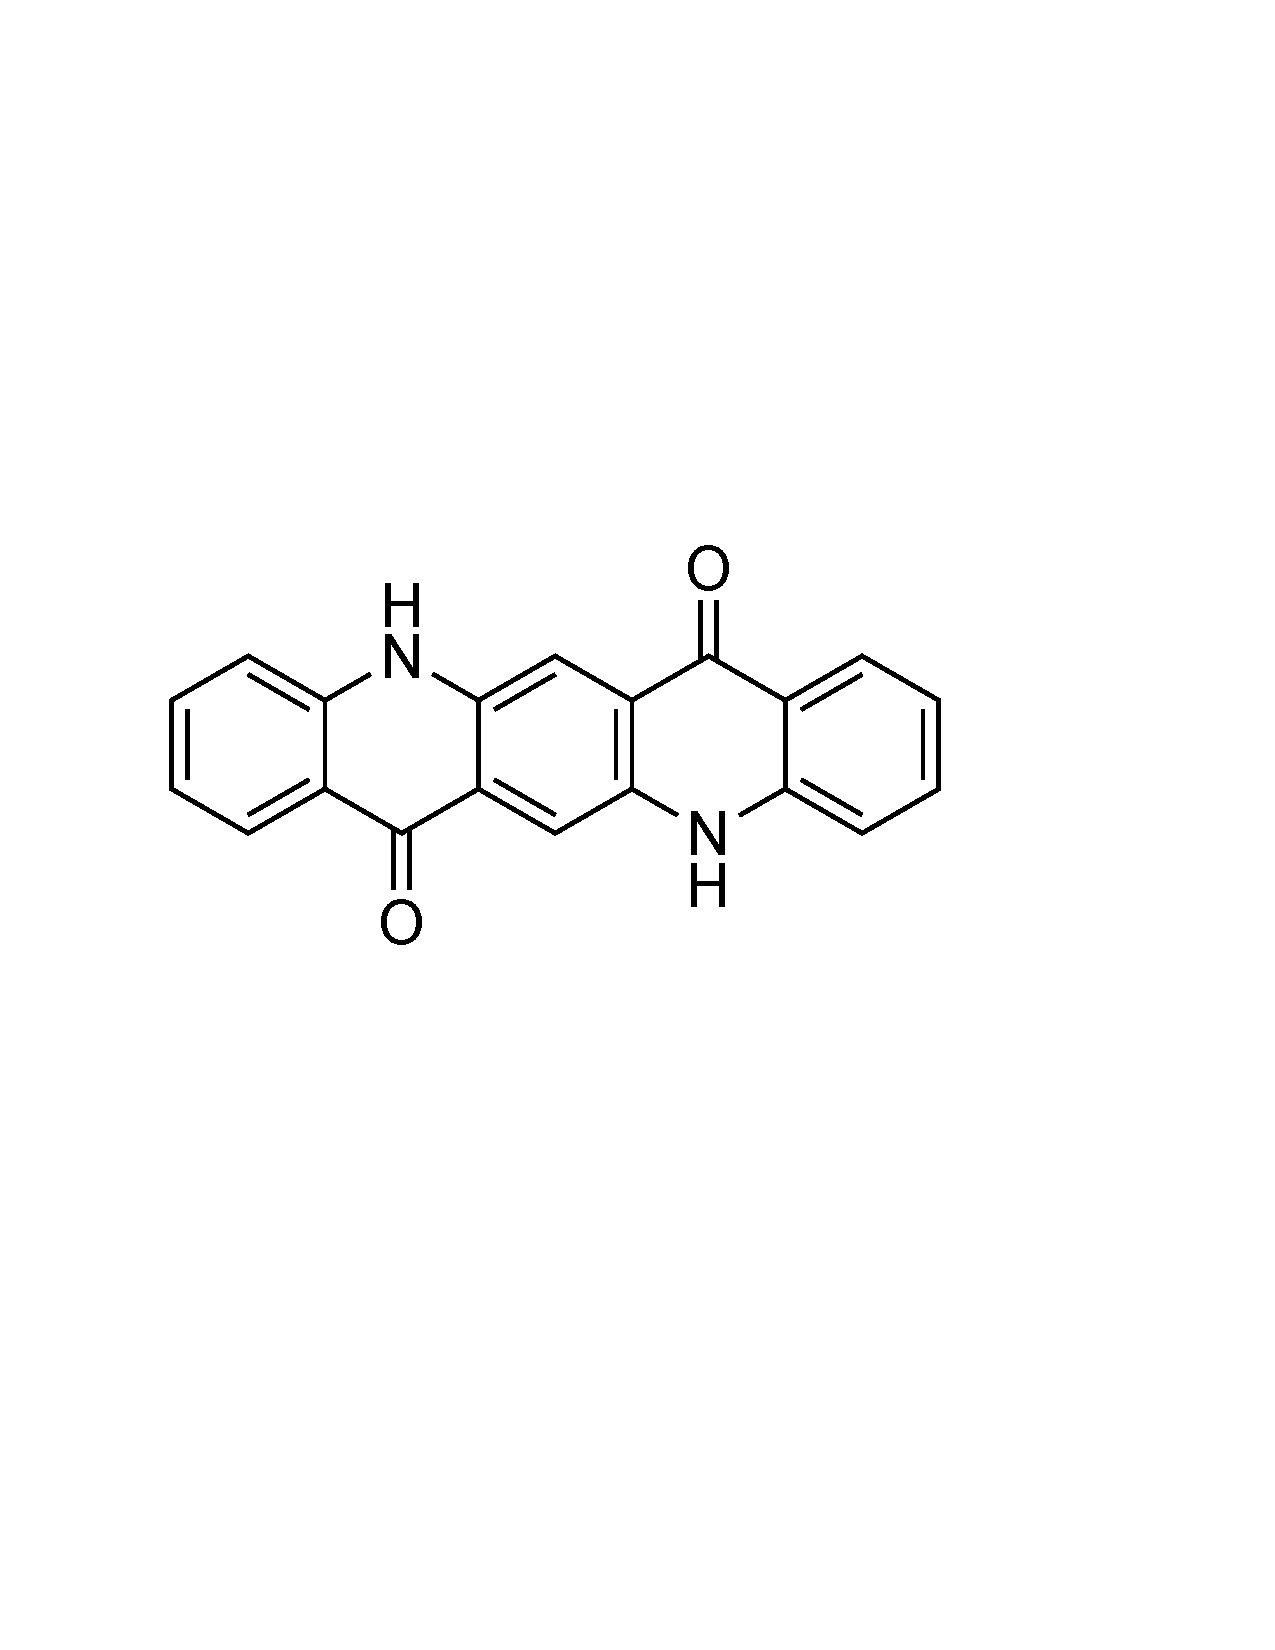
\includegraphics[width=\linewidth]{images/QA.pdf}
            \caption{Structure of QA.}
        \end{figure}
    \end{columns}
\end{frame}

\begin{frame}
    \frametitle{Multielectron processes in XPS}
    \begin{figure}
        \centering
        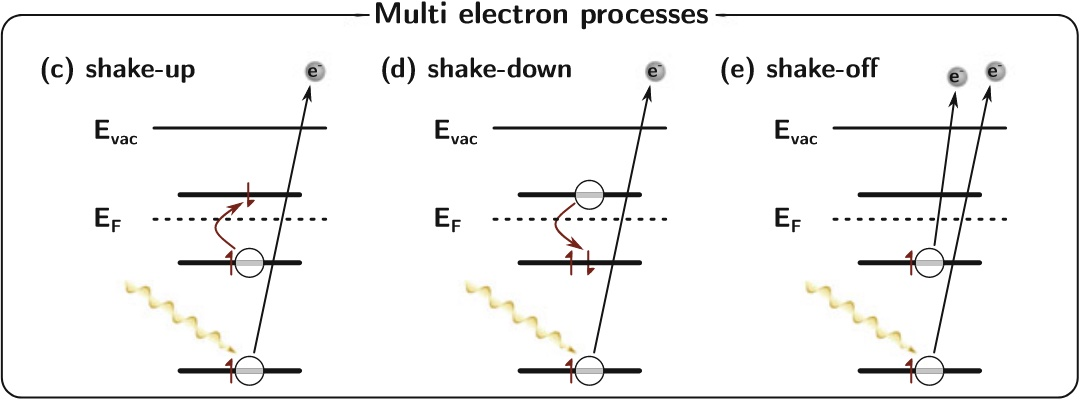
\includegraphics[width=\linewidth]{images/Satellites.jpg}
        \caption{Multielectron processes in XPS. Taken from \cite{Schlesinger2017}.}
    \end{figure}

\end{frame}

\begin{frame}{Literature Comparison}
    \begin{table}
        \centering
        \caption{Comparison of experimental results with literature values.}
        \footnotesize
        \begin{tabular}{@{}lccc@{}}
            \toprule
            \textbf{System} & \textbf{C$_{\text{arom}}$ BE (eV)} & \textbf{N1s BE (eV)} & \textbf{O1s BE (eV)} \\
            \midrule
            QA/$\alpha$-phase & 285.02 & 400.05 & 530.66 \\
            QA/$\beta$-phase & 284.55 & 399.87/397.66 & 530.68/530.19 \\
            PTCDA\autocite{Bauer2014} & 284.91 & - & 531.93 \\
            Indigo\autocite{Brunet2011, Michels2021,Xu2024} & 285.5 & 399.9 & 530.2 \\
            \bottomrule
        \end{tabular}
    \end{table}
    
    \vspace{1em}
    \begin{itemize}
        \item Good agreement with similar aromatic systems
        \item Large N1s shift consistent with deprotonation studies
        \item O1s values typical for carbonyl groups
        \item Phase transition shifts indicate stronger surface coupling
    \end{itemize}
\end{frame}

\begin{frame}{LEED Patterns}
    \begin{columns}[c]
        \column{0.5\textwidth}
        \begin{figure}
            \centering
            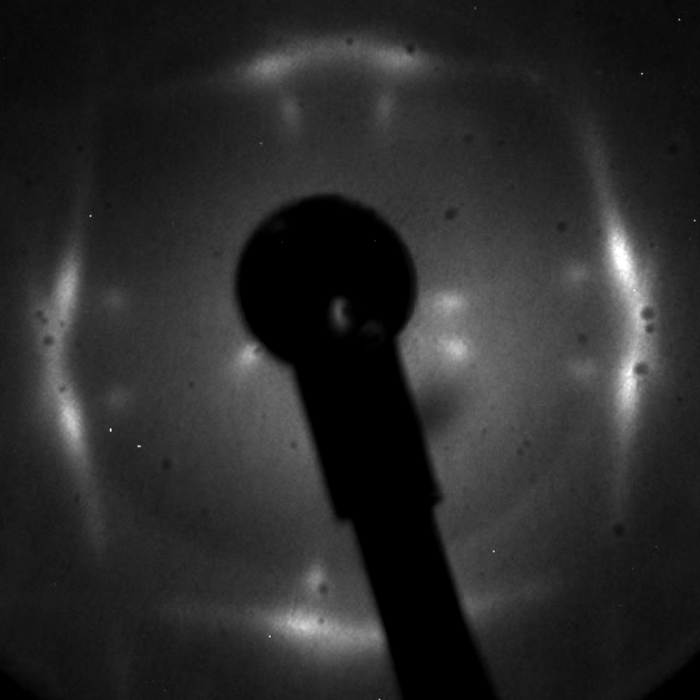
\includegraphics[width=0.8\linewidth]{images/LEED/LEED-alpha-25.5eV.png}
            \caption{Recorded LEED pattern of $\alpha$-phase at DLS.}
        \end{figure}
        
        \column{0.5\textwidth}
        \begin{figure}
            \centering
            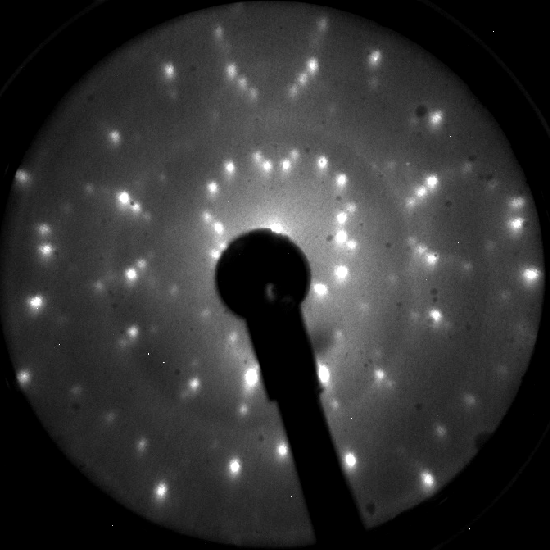
\includegraphics[width=0.8\linewidth]{images/LEED/LEED-beta-25.5eV.png}
            \caption{Recorded LEED pattern of $\beta$-phase at DLS.}
        \end{figure}
    \end{columns}
    
\end{frame}

\begin{frame}{Superstructure of QA on Ag(100)}
    \begin{columns}[c]
        \column{0.5\textwidth}
        \begin{itemize}
            \item \ac{POL} structure for $\alpha$-phase\autocite{Humberg2024} \\ $\rightarrow$ every point of superstructure falls on substrate lattice line in [10] direction
        \end{itemize}
        \begin{equation*}
        \mathbf{M_\alpha} =\begin{pmatrix}
        2 & 1.25 \\
        -3 & 4.80 
        \end{pmatrix}
        \end{equation*}

        \begin{itemize}
            \item $b_1=(6.8 \pm 0.1)~\si{\angstrom}$ 
            \item $b_2=(16.4 \pm 0.1)~\si{\angstrom}$ 
            \item $\alpha=90^\circ \pm 1^\circ$
        \end{itemize}

        
        \column{0.5\textwidth}
        \begin{itemize}
            \item Commensurate structure for $\beta$-phase\autocite{Humberg2024}
        \end{itemize}
        \begin{equation*}
        \mathbf{M_\beta} =\begin{pmatrix}
        4 & 3 \\
        -5 & 3 
        \end{pmatrix}
        \end{equation*}

        \begin{itemize}
            \item $b_1=(14.4 \pm 0.1)~\si{\angstrom}$ 
            \item $b_2=(16.8 \pm 0.1)~\si{\angstrom}$ 
            \item $\alpha=112^\circ \pm 1^\circ$
        \end{itemize}

    \end{columns}
\end{frame}

\begin{frame}{C1s spectra}
    \begin{figure}
        \centering
        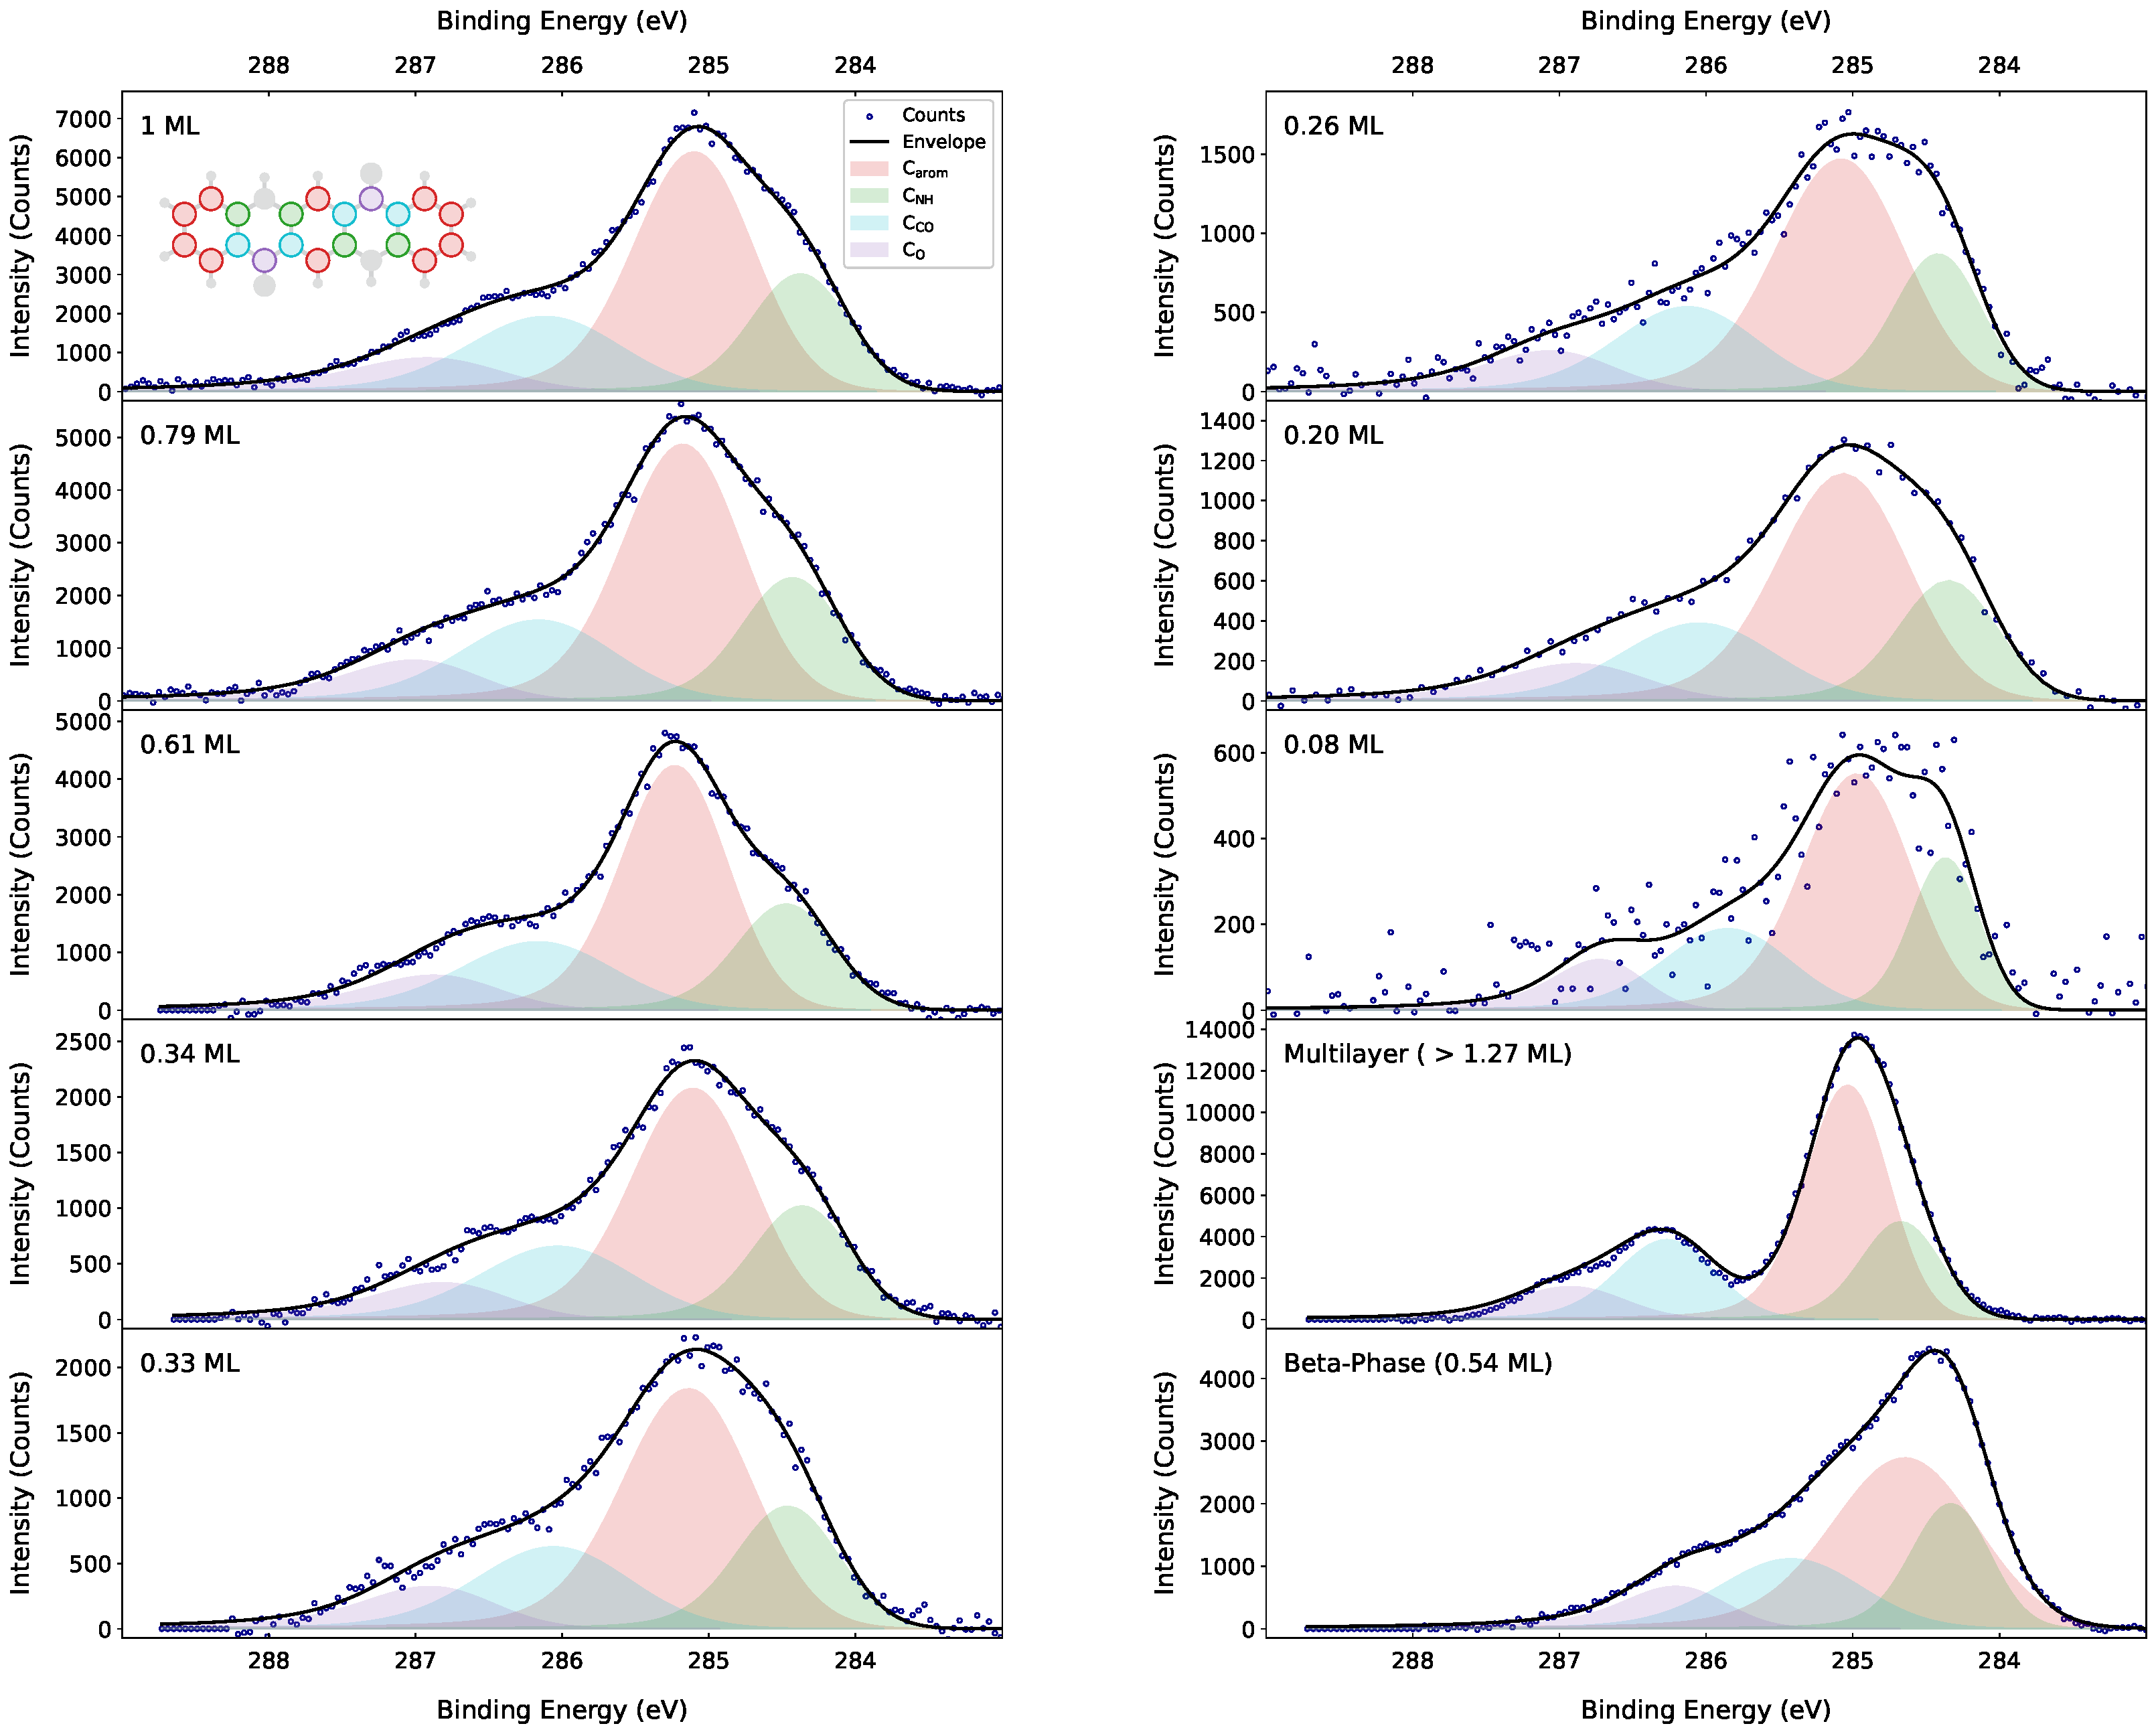
\includegraphics[height=0.8\textheight]{images/C1s-all.pdf}
        \caption{Overview of C1s XPS spectra for QA on Ag(100).}
    \end{figure}
\end{frame}

\begin{frame}{N1s spectra}
    \begin{figure}
        \centering
        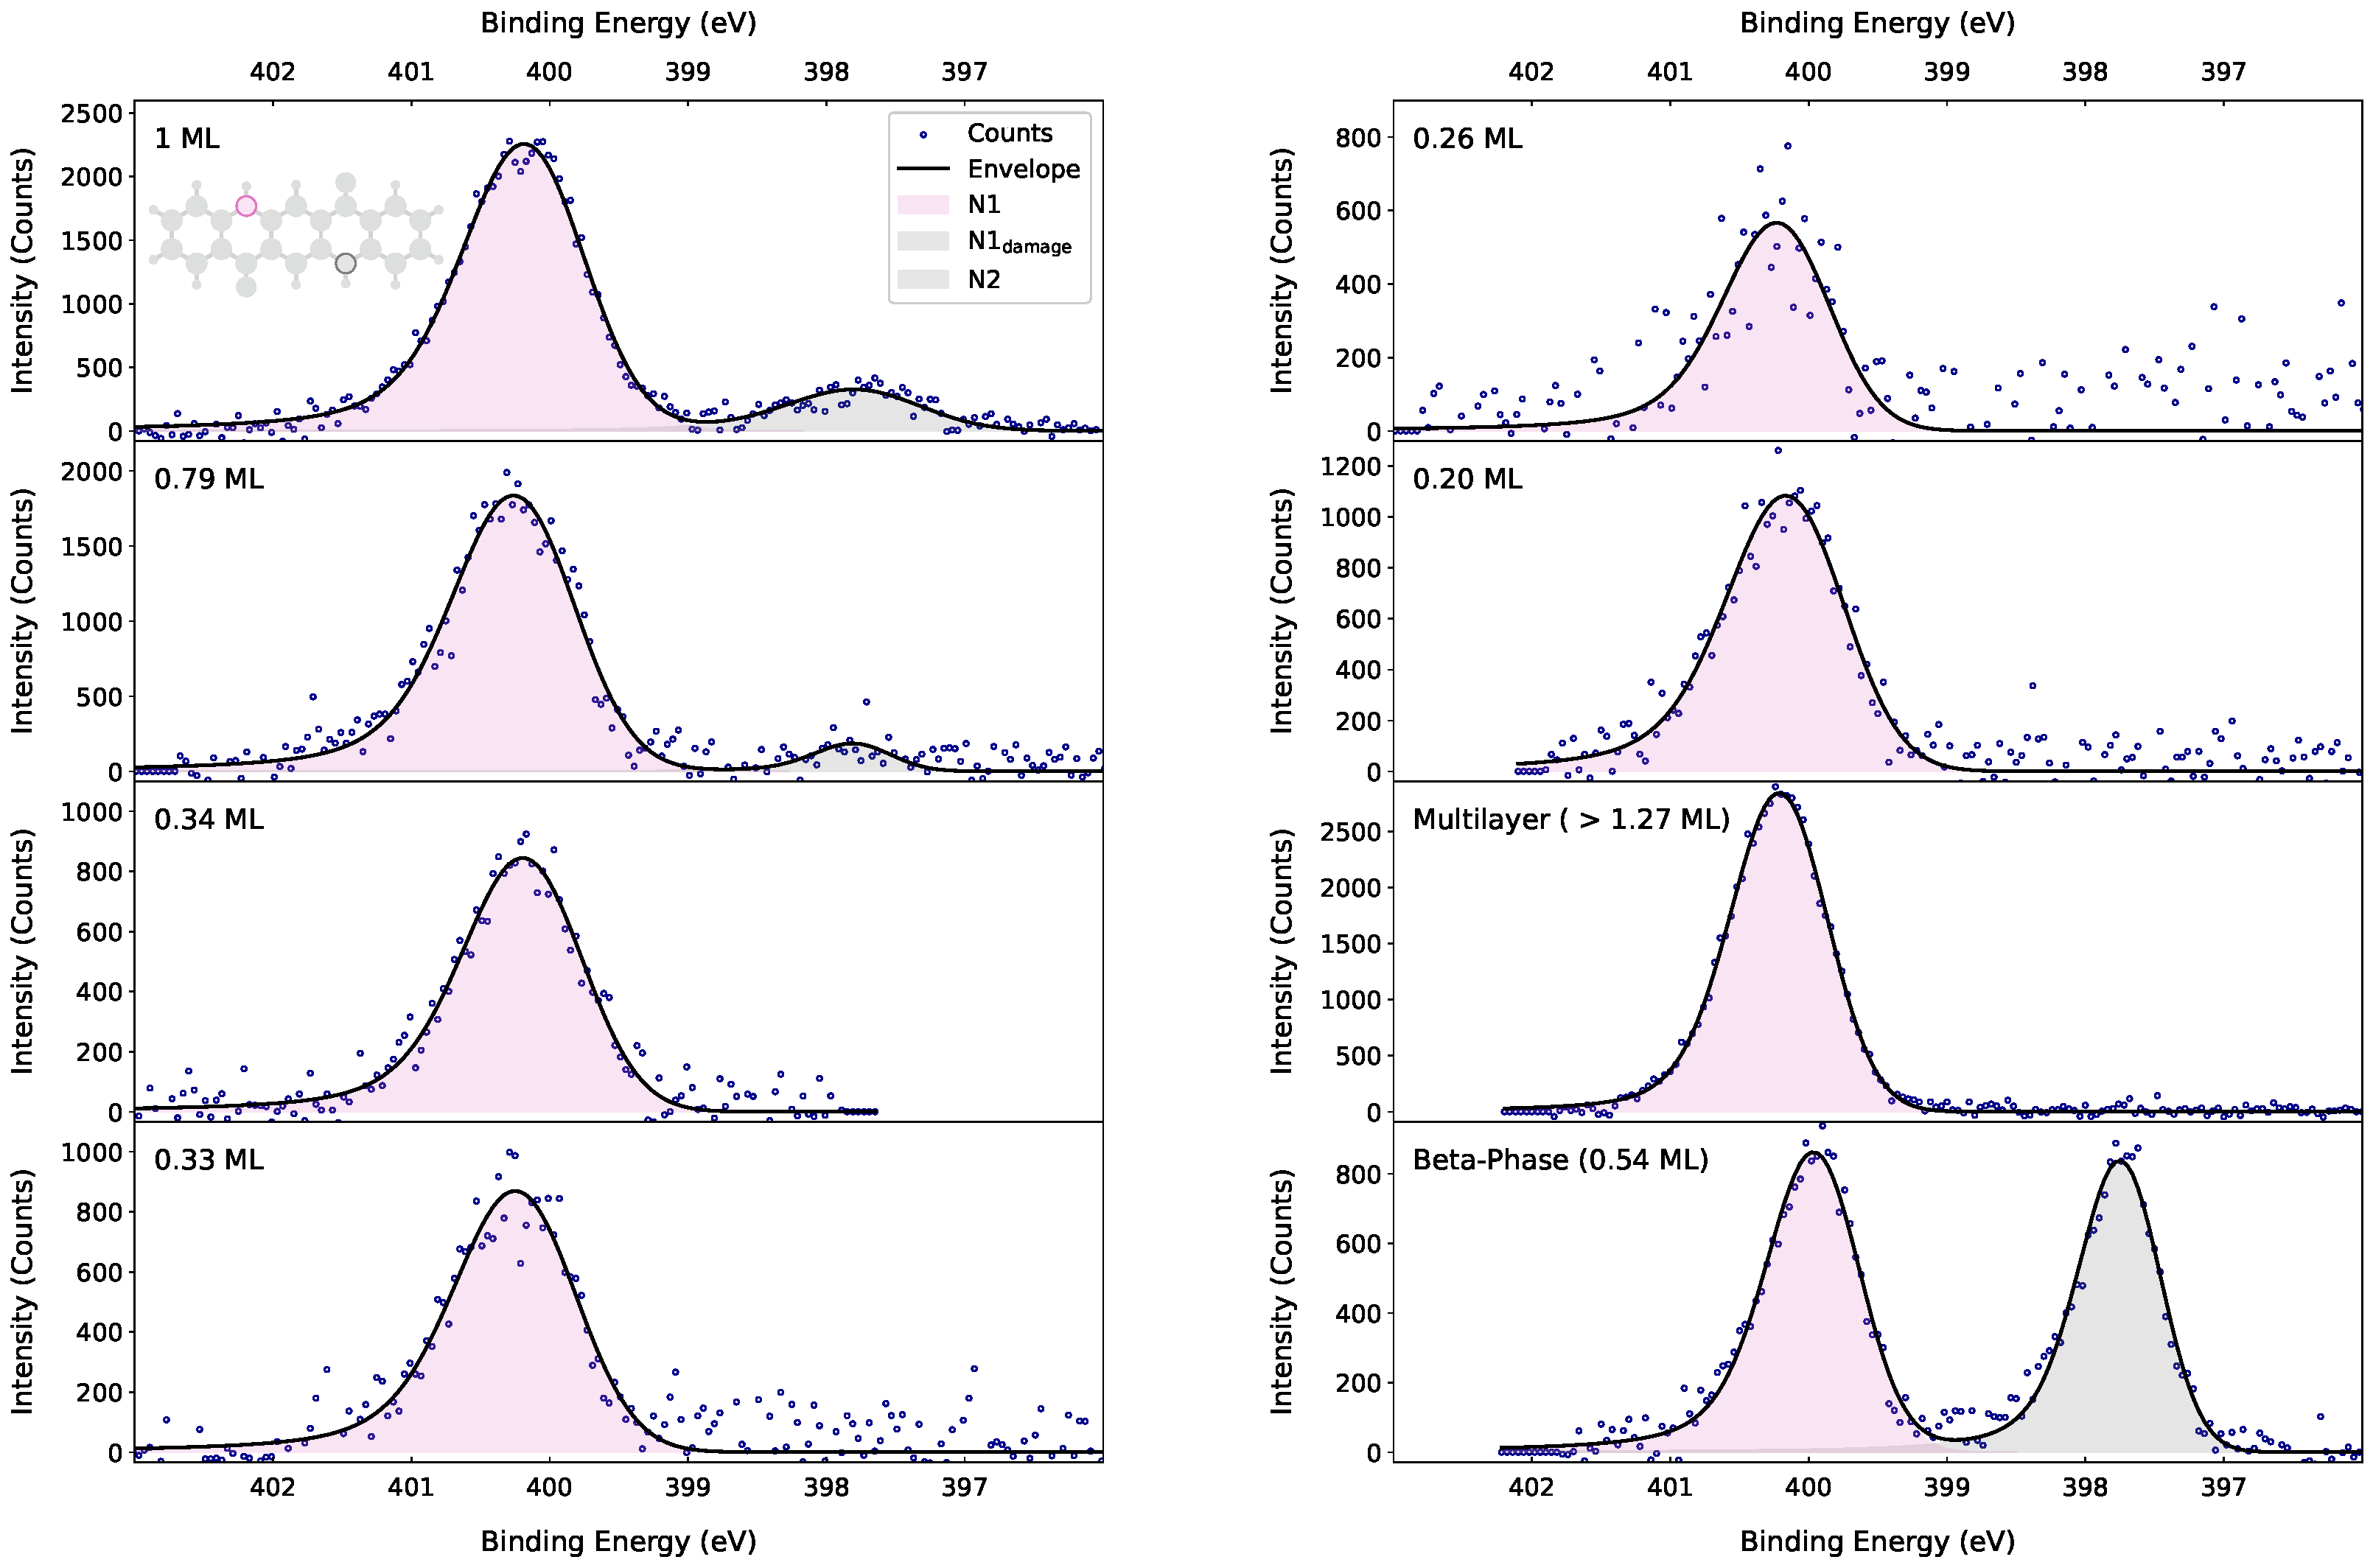
\includegraphics[height=0.8\textheight]{images/N1s-all.pdf}
        \caption{Overview of N1s XPS spectra for QA on Ag(100).}
    \end{figure}
\end{frame}

\begin{frame}{O1s spectra}
    \begin{figure}
        \centering
        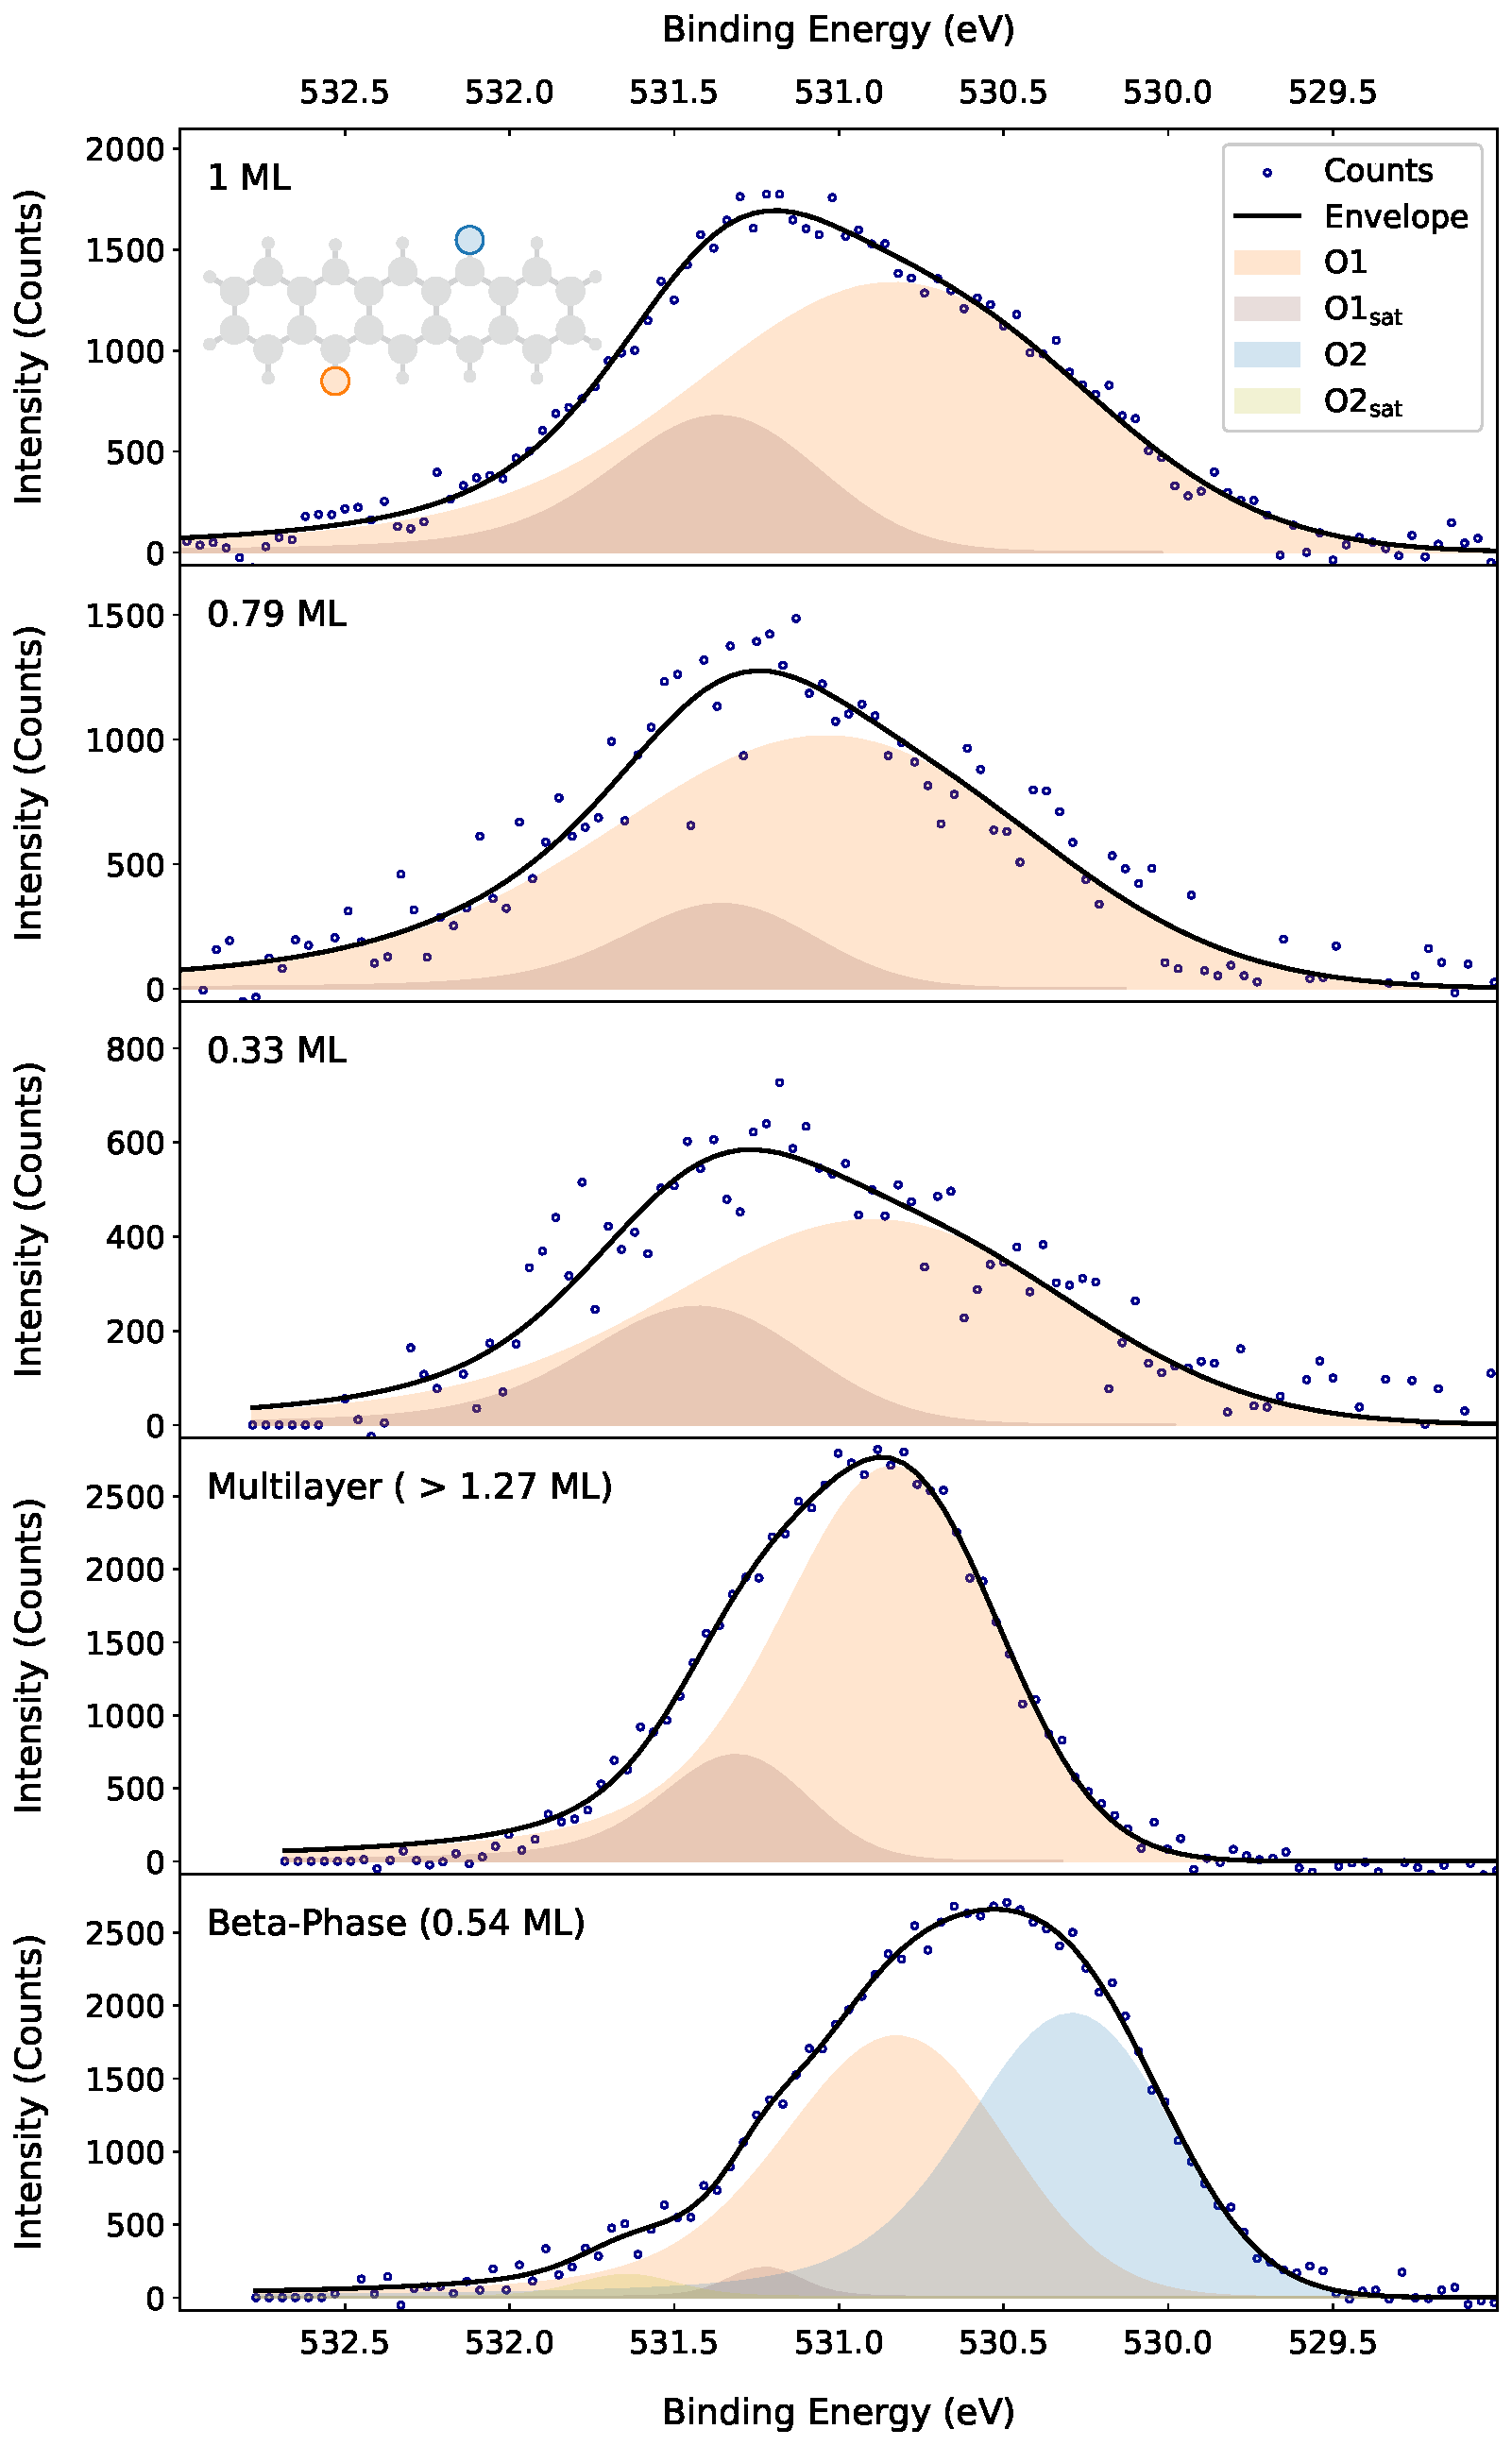
\includegraphics[height=0.8\textheight]{images/O1s-all.pdf}
        \caption{Overview of O1s XPS spectra for QA on Ag(100).}
    \end{figure}
\end{frame}


\begin{frame}{XPS fitting parameter}
   
    \begin{table}
	\centering
    \footnotesize
    \begin{tabular}{@{}ccc@{}} \toprule
        ~~~~~~peak~~~~~~ & ~~~~~~line shape~~~~~~ & ~~~~~~area ratio~~~~~~ \\
        \midrule
        $\mathrm{C_{arom}}$ & LA(1,8,800) & 10 \\
        $\mathrm{C_{NH}}$ & LA(1,8,800) & 4 \\
        $\mathrm{C_{CO}}$ & LA(1,8,800) & 4 \\
        $\mathrm{C_{O}}$ & LA(1,8,200) & 2 \\
        \midrule
        O1 & LA(1,8,400) & 1 (for $\beta$-phase) \\
        $\mathrm{O1_{sat}}$ & LA(1,1,400) & - \\
        O2 & LA(1,8,400) & 1 (for $\beta$-phase) \\
        $\mathrm{O2_{sat}}$  & LA(1,1,400) & - \\
        \midrule
        N1 & LA(1,8,400) & 1 (for $\beta$-phase) \\
        $\mathrm{N1_{damage}}$  & LA(1,8,400) & - \\
        N2 & LA(1,8,400) & 1 (for $\beta$-phase) \\
        \bottomrule
    \end{tabular}
    \end{table}

\end{frame}


\begin{frame}{Parameters of XPS fits}
    \begin{table}
    \centering
    \scriptsize
        \begin{tabular}{@{}lcccccc@{}}
            \toprule
            \textbf{Phase} & \textbf{Core-level} & \textbf{Component} & \textbf{BE (eV)} & \textbf{FWHM (eV)} & \textbf{Area} \\
            \midrule
            $\alpha$ & C1s & C$_{\text{arom}}$ & 285.02 & 0.94 & 10 \\
            &  & C$_{\text{NH}}$ & 284.31 & 0.76 & 4 \\
            &  & C$_{\text{CO}}$ & 286.01 & 1.20 & 4 \\
            &  & C$_{\text{O}}$ & 286.72 & 1.15 & 2 \\
            \cmidrule{2-6}
            & N1s & N1 & 400.05 & 1.02 & -  \\
            &  & N1$_\text{damage}$ & 397.66 & 1.16 & -  \\
            \cmidrule{2-6}
             & O1s & O1 & 530.66 & 1.36 & -  \\
            &  & O1$_\text{sat}$ & 531.27 & 0.71 &  -  \\
            \midrule \midrule
            $\beta$ & C1s & C$_{\text{arom}}$ & 284.55 & 1.13 & 10 \\
            &  & C$_{\text{NH}}$ & 284.28 & 0.62 & 4 \\
            &  & C$_{\text{CO}}$ & 285.32 & 1.11 & 4 \\
            &  & C$_{\text{O}}$ & 286.07 & 0.79 & 2 \\
            \cmidrule{2-6}
            & N1s & N1 & 399.87 & 1.20 & 1 \\
            &  & N2 & 397.66 & 1.20 & 1 \\
            \cmidrule{2-6}
            & O1s & O1 & 530.68 & 0.71 & 1 \\
            &  & O1$_\text{sat}$ & 531.20 & 0.45 &  -  \\
            &  & O2 & 530.19 & 0.68 & 1 \\
            &  & O2$_\text{sat}$ & 531.66 & 0.36 &  -  \\
            \bottomrule
        \end{tabular}
    \end{table}

\end{frame}

\end{document}